\chapter{Appendix of ``Reelection Backfire: \\ How Reelection Concerns Affect the Delegation of Public Security Policy in Mexico''\label{chap:append1}}



%%%%%%%%% Electoral Reform 2014
\section{Political Background of the 2014 Electoral Reform}\label{appendix:reform_backgorund}

It is important to understand the electoral reform political motivation, which involved a bargaining process with the opposition as well as the incorporation of pending laws from the political reform of 2012 under the PAN presidency. In the last year of Felipe Calderon presidency, a political reform was introduced in Congress including a term limit removal for all political actors. This reform was proposed and introduced during the electoral period of that year, increasing political tensions among the incumbent and opposition parties. The PRI -at the time part of the opposition and in control of the lower legislative house- blocked the reform and targeted reelection and the introduction of a second electoral round for the presidential election. 
 
  The 2012 presidential election was won by the coalition ``Alliance for Mexico'' with its presidential candidate Enrique Pena Nieto.\footnote{The PRI won with 38.2\% of total votes, followed by the PRD with 32.6\% and the PAN with 25.390\%.} However, the election suffered multiple electoral irregularities exposed by the national media. Among anomalies, opposition parties led by Andres Manuel Lopez Obrador -the second runner of presidential election and at the time presidential candidate for the left-wing party PRD-, argued PRI's financial expenses above campaign caps and vote-buying practices including the distribution of gift cards from several institutions, including one of the country's largest supermarket chains, Soriana, to voters in the State of Mexico and Mexico city. \citet{cantu_2019} finds not only an effect of the gift cards in PRI electoral return, but a magnitude that increases given proximity of electoral precincts to stores. While the special commission in the Chamber of Deputies found that the PRI invested \$5,200 million pesos in the campaign, an amount 15 times larger than the finance cap of \$336 million pesos, and the Inspection Unit from the Federal Electoral Institute (IFE for its acronym in Spanish) detailed the financing network where Soriana, Banamex, Monex and other firms where involved, the Unit did not point to any law violation. Without a public discussion, the ministers of the Federation Judicial Electoral Tribunal (TEPJF for its acronym in Spanish) deemed the appeal filed by the PRD unfounded and endorsed IFE's  criterion that the PRI was not obliged to register the agreement with Soriana, Banamex or Monex as campaign expenses.\footnote{In his presentation, magistrate Manuel Gonzalez Oropeza stated that the analysis carried by the Inspection Unit showed that ``neither the allegedly hidden financing was accredited individually or jointly" by any member of the PRI. See \url{https://www.jornada.com.mx/2013/01/24/politica/013n2pol} for more detail.} The final resolution of IFE's Council and the TEPJF increased citizens and opposition mistrust on electoral institutions. 

By early 2013, the Pena Nieto administration pushed an aggressive set of reforms to privatize the energy sector and modify the existent fiscal institutions in the country. To increase the probability of success, the PRI with the PAN and PRD, the three main political parties at the time, lead the construction of the Mexican Pact Accord, a series of roundtables intended to negotiate the energy sector reform along a set of structural reforms that had fail to pass through congress due to political gridlocks.\footnote{The PRD was no longer under the Lopez Obrador leadership who left the party to build a new left-wing party called MORENA once the leaders from the PRD agreed to form part of the Mexican Pact Accord.} While the Electoral Reform was not under PRI's set of desired reforms, the opposition utilize it as a bargaining chip to approve those pursued by the PRI \citep{zamitiz_2017}. By the end of May 2013, a roundtable to discuss the electoral reform was installed. Specifically, commitment 94 of the Pact Accord introduced reelection for discussion. However, due to lack of consensus, the Mexican Pact Accord did not submit an electoral reform proposal to Congress and left the bargaining process to the Senate. Two months later, on July 24, 2013, PAN and PRD pushed a political-electoral reform with 36 law changes that included  the creation of a National Electoral Institute (INE for its acronym in Spanish) that would be in charge of federal, state and local elections and reelection for federal and local legislators and mayors. In the words of the current Chairman of the INE, Lorenzo Cordova, ``[w]ith the reform, we went from an electoral model made up of a federal electoral system and thirty-two electoral systems, to a national election system in which a national authority and thirty-two local authorities coexist; a national administrative body was created, with clear powers and powers for local elections, and an authority was created that coordinates and guarantees the same parameters for the application of laws by local authorities, in order to standardize the conditions of the electoral competition in all elections and to promote a more transparent and impartial democracy throughout the country.\footnote{From Cfr. Compendio de Legislacion Nacional Electoral, Mexico, INE, FEPADE, UNAM, TEPJF, Tomo II, 2014, p. XXXIX.} 


The reaction of governors was not smooth since reelection would limit the influence of governors and local elites on the electoral processes of the 32 states. Strong governors like the priista Eruviel Avila Villegas from the State of Mexico labeled this initiative as ``democratic regression".\footnote{For more detail see ``Regresion democratica, creacion del Instituto Nacional de Elecciones, La Jornada, 30 de octubre, 2013, p. 15. \url{https://www.20minutos.com.mx/noticia/b82075/regresion-democratica-creacion-del-instituto-nacional-de-elecciones/}} Given the state-level opposition, Senate leaders from the PAN and PRD chose to approve the electoral reform in December 2, 2013, before the energy reform, and thus increased their political grip over the PRI.\footnote{The electoral reform approved by the Senate included reelection for federal legislators and governors for up to 12 years, as well as reelection for local legislators and mayors. Congress, however, modified the proposal removing governors reelection. The electoral reform was approved with 408 votes in favor and 69 against in Congress on December 3, 2013, and weeks later by the Senate due to modifications of the original reform project.} By January 2014, PAN and PRD threatened to back the energy reform  if the PRI did not push local state legislatures from approving the electoral reform, a constraint imposed by the Mexican constitution, which at the time where blocking the reform given pressure from various PRI governors.\footnote{For more detail see Enrique Mendez, ``PAN: estancados, cambios en materia politica por presion de los gobernadores, La Jornada, 9 de enero de 2014, p. 5., \url{https://jornada.com.mx/2014/01/09/politica/005n3pol}.} The political gridlock led former President Pena Nieto to ``exhort" local legislators to approve the electoral reform. On January 31, 2014, the reform was promulgated by the President and contained three main changes: (1) the creation of the INE; (2) removal of term limits of mayors, local and federal legislators for up to 2 terms; (3) the introduction of a ``party-lock"	where mayors or legislators who wish to reelected could not switch parties. As a result, while voter accountability increased, party control remained unchanged since candidate nominations and campaign funding still depended strongly on them. 

%%%%%%%%%%%%%%%%%%%%%%%%%%%%%%%%%%%%

%\renewcommand{\thetable}{B-\arabic{table}}
%\setcounter{table}{0}
 
% \renewcommand{\thefigure}{B-\arabic{figure}}
%\setcounter{figure}{0}

\section{Additional Tables and Figures \label{sec:additional_tables}}

\subsection{Descriptive Statistics}

%Table
\begin{table}[H]
\centering 
\caption{Descriptive statistics}
 
\label{tab:descriptive}
\scalebox{0.5}{ 
{
\def\sym#1{\ifmmode^{#1}\else\(^{#1}\)\fi}
\begin{tabular}{l*{1}{ccccc}}
\hline\hline
            &        \textbf{Mean}&  \textbf{SD}&  \textbf{Min}&  \textbf{Max}& \textbf{N}\\
\hline
\emph{Pane A - Security Cooperation Agreements:} 	&		&		&		&		\\
Security Coop. Agreement with governor&        0.28&        0.45&           0&           1&      17,832\\
Security Coop. Agreement with other actors besides the governor&        0.06&        0.24&           0&           1&       6,466\\
Delegate Public Security Provision&        0.29&        0.45&           0&           1&       7,123\\
Delegate Transit Activities&        0.10&        0.30&           0&           1&       7,123\\
Delegate Training of Police Forces&        0.08&        0.27&           0&           1&       4,750\\
Delegate Equipment and Technology&        0.08&        0.26&           0&           1&       4,750\\
Delegate Research Activities&        0.07&        0.26&           0&           1&       4,750\\
Delegate Intelligence Activities&        0.07&        0.26&           0&           1&       4,750\\
Delegate the Unification of Laws and Procedures&        0.08&        0.27&           0&           1&       4,750\\
Delegate Public Security Prevention&        0.08&        0.27&           0&           1&       4,750\\
Reason to delegate: Constitutional Change&        0.12&        0.33&           0&           1&      14,248\\
Reason to delegate: Change in Local Laws&        0.11&        0.31&           0&           1&      14,248\\
Reason to delegate: Constitutional Change&        0.11&        0.31&           0&           1&      14,248\\
Reason to delegate: Need of Professionalization&        0.12&        0.33&           0&           1&      14,248\\
Reason to delegate: Need of Coordination&        0.17&        0.38&           0&           1&      14,248\\
Reason to delegate: Prevalence of Crime&        0.09&        0.29&           0&           1&      14,248\\
Reason to delegate: Other&        0.07&        0.25&           0&           1&      14,248\\


\\
\emph{Panel B - Violence:} 	&		&		&		&		\\
deaths by homicide per capita (INEGI)&       23.99&      128.24&           0&       8,462&      21,375\\
log(deaths by homicide per capita) (INEGI)&       -8.34&        1.04&         -13&        -2.4&      21,375\\
asinh(deaths by homicide per capita) (INEGI)&        2.33&        1.91&           0&         9.7&      21,375\\

\\
\emph{Panel C - Citizens' Preferences:} 	&		&		&		&		\\
Topic that worries most: narcotraffic (for all years)&        0.15&        0.05&           0&         .37&      16,625\\
Topic that worries most: insecurity (for all years)&        0.56&        0.09&           0&         .77&      16,625\\
Topic that worries most: punishment of criminals (for all years)&        0.17&        0.06&           0&         .38&      16,625\\
Topic that worries most: corruption (for all years)&        0.26&        0.04&           0&         .36&      16,625\\
Topic that worries most: poverty (for all years)&        0.34&        0.07&           0&         .52&      16,625\\
Topic that worries most: unemployment (for all years)&        0.40&        0.07&           0&         .57&      16,625\\
Topic that worries most: inflation (for all years)&        0.35&        0.04&           0&         .46&      16,625\\
Topic that worries most: natural disaster (for all years)&        0.05&        0.02&           0&         .12&      16,625\\
Topic that worries most: water scarcity (for all years)&        0.15&        0.04&           0&         .25&      16,625\\
Topic that worries most: health (for all years)&        0.23&        0.03&           0&         .31&      16,625\\
Topic that worries most: education (for all years)&        0.31&        0.05&           0&         .47&      16,625\\

\\
\emph{Panel D - Incumbents' quality:} 	&		&		&		&		\\
Incumbent undergraduate or graduate title (indicator)&        0.06&        0.24&           0&           1&      19,430\\

\\ 
%\emph{Pane B - 2014 Electoral Reform:} 	&		&		&		&		\\
%Lag 8               &        0.01&        0.12&           0&           1&      20,710\\
Lag 7               &        0.02&        0.13&           0&           1&      20,710\\
Lag 6               &        0.06&        0.23&           0&           1&      20,710\\
Lag 5               &        0.10&        0.30&           0&           1&      20,710\\
Lag 4               &        0.10&        0.30&           0&           1&      20,710\\
Lag 3               &        0.10&        0.30&           0&           1&      20,710\\
Lag 2               &        0.10&        0.30&           0&           1&      20,710\\
Lag 1               &        0.10&        0.30&           0&           1&      20,710\\
Reform, time 0      &        0.10&        0.30&           0&           1&      20,710\\
Lead 1              &        0.10&        0.30&           0&           1&      20,710\\
Lead 2              &        0.09&        0.28&           0&           1&      20,710\\
Lead 3              &        0.08&        0.28&           0&           1&      20,710\\


%\\

\\ 
 

\hline\hline
\multicolumn{6}{p{1.3\textwidth}}%{\footnotesize{Note: .        
 % }} \\  

\end{tabular} 
} 
}
\end{table}

\pagebreak

%Table
\begin{table}[H]
\centering 
\caption{Descriptive statistics (continuation)}
 
\label{tab:descriptive2}
\scalebox{0.5}{ 
{
\def\sym#1{\ifmmode^{#1}\else\(^{#1}\)\fi}
\begin{tabular}{l*{1}{ccccc}}
\hline\hline
            &        \textbf{Mean}&  \textbf{SD}&  \textbf{Min}&  \textbf{Max}& \textbf{N}\\
\hline

\emph{Panel E - Mechanisms:} 	&		&		&		&		\\
Topic that worries most: narcotraffic (average pre-treatment)&        0.15&        0.05&           0&         .27&      21,375\\
Topic that worries most: insecurity (average pretreatment)&        0.52&        0.08&           0&         .68&      21,375\\
Topic that worries most: punishment of criminals (average pretreatment)&        0.12&        0.02&           0&         .19&      21,375\\
Topic that worries most: poverty (average pretreatment)&        0.37&        0.07&           0&          .5&      21,375\\
Topic that worries most: unemployment (average pretreatment)&        0.46&        0.04&           0&         .52&      21,375\\
Topic that worries most: inflation (average pretreatment)&        0.37&        0.03&           0&         .41&      21,375\\
Topic that worries most: natural disaster (average pretreatment)&        0.05&        0.01&           0&        .088&      21,375\\
Topic that worries most: water scarcity (average pretreatment)&        0.15&        0.03&           0&          .2&      21,375\\
Topic that worries most: corruption (average pretreatment)&        0.24&        0.04&           0&         .34&      21,375\\
Topic that worries most: health (average pretreatment)&        0.24&        0.03&           0&         .29&      21,375\\
Topic that worries most: education (average pretreatment)&        0.31&        0.06&           0&          .4&      21,375\\
Trust in Municipal Security Forces&        0.21&        0.05&           0&          .4&      21,375\\
Trust in State Security Forces&        0.22&        0.05&           0&         .37&      21,375\\
Trust in Federal Security Forces, including the military&        0.55&        0.16&           0&         .77&      21,375\\
Identify Municipal Security Forces&        0.70&        0.06&           1&         .87&      21,375\\
Identify State Security Forces&        0.51&        0.07&           0&          .7&      21,375\\
Identify Federal Security Forces, including the military&        0.53&        0.08&           0&         .75&      21,375\\
Corruption of Municipal Security Forces&        1.24&        0.15&           1&         1.7&      21,375\\
Corruption of State Security Forces&        1.24&        0.14&           1&         1.6&      21,375\\
Corruption of Federal Security Forces, including the military&        1.07&        0.14&           1&         1.6&      21,375\\
Efficiency of Municipal Security Forces&        0.24&        0.06&           0&         .42&      21,375\\
Efficiency of State Security Forces&        0.25&        0.06&           0&         .41&      21,375\\
Efficiency of Federal Security Forces, including the military&        0.57&        0.15&           0&         .78&      21,375\\
Detained by local police per capita (in flagrancy, SNSP)&       10.29&      133.10&           0&      11,408&      21,375\\
log(Detained by local police per capita) (in flagrancy, SNSP)&       -9.06&        1.32&         -14&        -2.2&      21,375\\
log(heroine kg), SEDENA&        0.01&        0.15&           0&         5.4&      21,375\\
log(meth kg), SEDENA&        0.05&        0.48&           0&          10&      21,375\\
log(cocaine kg), SEDENA&        0.04&        0.36&           0&         7.8&      21,375\\
log(poppy kg), SEDENA&        0.19&        0.82&           0&         8.8&      21,375\\
log(laboratories erradicated), SEDENA&        0.02&        0.17&           0&         4.1&      21,375\\
 
\\
\emph{Panel F - Controls:} 	&		&		&		&		\\
Population (INEGI and CONAPO projections)&      49,233&     129,415&         409&   1,714,709&       2,247\\
 
Winning margin: first - second runner (governor)&        0.15&        0.13&           0&           1&      24,470\\
Party alignment with federal executive=1; 0 otherwise&        0.54&        0.50&           0&           1&      24,470\\

\\ 
 
    
\hline\hline
\multicolumn{6}{p{1.3\textwidth}}%{\footnotesize{Note: .        
 % }} \\  

\end{tabular} 
} 
}
\end{table}
\clearpage
\subsection{Main Results}
\begin{table}[H]\def\sym#1{\ifmmode^{#1}\else\(^{#1}\)\fi}
\centering
\caption{Effect of 2014 Term Limit Reform on Security Cooperation Agreements signed with the Governor, 2010-2018}
\label{tab:as_agreements}
\scalebox{0.75}{
\begin{tabular}{lcc}
\hline \hline
\\ \multicolumn{3}{l}{Dependent variable:}\\
& \multicolumn{2}{c}{Security Cooperation Agreement} \\
& \multicolumn{2}{c}{w/ Governor$^{a}$} \\

& \multicolumn{1}{c}{(1)} & \multicolumn{1}{c}{(2)} \\
\cmidrule(lrr){2-2}  \cmidrule(lrr){3-3}\\
\addlinespace
Lag 7 years &      $ 0.1123^{} $ &  $ 0.1123^{} $   \\
& ($ 0.1709$) & ($ 0.7117 $) \\
Lag 6 years &          $ -0.0383^{} $ &   $ -0.0383^{} $  \\
& ($ 0.0579$) & ($ 0.2458 $) \\
Lag 5 years &        $ -0.0848^{} $ &   $ -0.0848^{} $ \\
& ($ 0.0846$) & ($ 0.2404 $) \\
Lag 4 years &         $ 0.0751^{} $ &      $ 0.0751^{} $  \\
& ($ 0.3174$) & ($ 0.2890 $) \\
Lag 3 years &        $ 0.2088^{} $ &     $ 0.2088^{} $ \\
& ($ 0.2603$) & ($ 0.2139 $) \\
Lag 2 years &        $ 0.0044^{} $ &    $ 0.0044^{} $  \\
& ($ 0.1583$) & ($ 0.2139 $) \\
Reform, time 0 &        $ -0.2446^{***} $ &     $ -0.2446^{***} $ \\
& ($ 0.0475$) & ($ 0.0685 $) \\
Lead 1 year &         $ -0.4154^{***} $ &       $ -0.4154^{***} $ \\
& ($ 0.0610$) & ($ 0.0610 $) \\
Lead 2 years &         $ -0.4259^{***} $ &      $ -0.4259^{***} $  \\
& ($ 0.0571$) & ($ 0.0571 $) \\
Lead 3 years &        $ -0.5931^{***} $ &     $ -0.5931^{***} $ \\
& ($ 0.0604$) & ($ 0.0604 $) \\
\addlinespace
Observations       &                 12,173        &          12,173  \\
R-squared        &              0.4545        &           0.4545   \\
Mun. FEs       &     \checkmark         &  \checkmark    \\
Year. FEs       &     \checkmark         &  \checkmark   \\
Controls$^b$   &      \checkmark       &      \checkmark    \\
Cohort weighted   &   \checkmark       &   \checkmark    \\
WILD CI   &          &   \checkmark    \\
Aggregate effect        &           $   -0.4197^{***} $        &           $-0.4197^{***} $    \\
SE (aggregate eff.)        &              0.0457        &           0.0473   \\
\hline \hline
\multicolumn{3}{p{0.6\textwidth}}{\footnotesize{Notes: Coefficients show IW estimators following \citet{abraham_sun_2020}. Two relative time periods (lag 8 and 1) are removed to avoid collinearity problems noted by \citet{abraham_sun_2020}. Standard errors in parentheses are clustered at the state level, with the following significance-level: $^{***}$ 1\%; $^{**}$ 5\%; and $^*$ 10\%, that refer to two-sided t-test with the null hypothesis equal to 0 for each relative time period. $^a$ Refers to security cooperation agreements signed with the Governor. $^b$ Pretreatment controls include: governor winning margin; party alignment with the President;  party alignment with the Governor; municipal winning margin; logged population; logged organized crime related deaths; and Cartel presence.}} \\
\end{tabular}
} 
\end{table}
    
 
 \clearpage
\subsection{Robustness}

\begin{table}[htbp]\def\sym#1{\ifmmode^{#1}\else\(^{#1}\)\fi}
\centering
\caption{Effect of 2014 Term Limit Reform on Signing Security Cooperation Agreements, Average Effect }
\label{tab:as_aggregate}
\scalebox{0.65}{
\begin{tabular}{lcccc}
\hline \hline
\\ \multicolumn{3}{l}{Dependent variable: Sign Security Cooperation Agreement w/ Governor}\\
Model: & CATTs & CATTs w/ WILD CIs & Change ref. period (t=0) & Trim $<$ t-4 \\
& \multicolumn{1}{c}{(1)} & \multicolumn{1}{c}{(2)} & \multicolumn{1}{c}{(3)}  & \multicolumn{1}{c}{(4)}  \\
\cmidrule(lrr){2-2}  \cmidrule(lrr){3-3}  \cmidrule(lrr){4-4} \cmidrule(lrr){5-5}\\
\addlinespace
Reform Average Effect (from t to t+3)       & $-0.4197^{***} $ & $-0.4197^{***} $ & $-0.4622 ^{**} $ & $-0.3559^{***} $   \\
& (0.0457) & (0.0473)  & (0.1977) & (0.0468)  \\
\addlinespace
Observations       &      12,173 &      12,173 &      12,173 &      12,173 \\
R-squared         & 0.4545 & 0.4545 & 0.4545 & 0.4544 \\
Mun. FEs       &     \checkmark         &  \checkmark &     \checkmark         &  \checkmark     \\
Year. FEs       &     \checkmark         &  \checkmark  &     \checkmark         &  \checkmark \\
Controls$^b$   &      \checkmark       &      \checkmark &      \checkmark       &      \checkmark    \\
Cohort weighted   &   \checkmark       &   \checkmark  &   \checkmark       &   \checkmark  \\
Parallel trend holds   &   \checkmark       &   \checkmark  &   \checkmark       &   \checkmark   \\
\hline \hline
\multicolumn{5}{p{1.4\textwidth}}{\footnotesize{Notes: Coefficients show IW estimators following \citet{abraham_sun_2020}. Two relative time periods (lag 8 and 1) are removed to avoid collinearity problems noted by \citet{abraham_sun_2020} except for the specification that trims periods prior to t-4. Standard errors in parentheses are clustered at the state level, with the following significance-level: $^{***}$ 1\%; $^{**}$ 5\%; and $^*$ 10\%, that refer to two-sided t-test with the null hypothesis equal to 0 for each relative time period. $^b$ State-level controls include governor winning margin in last pre-treatment election and an indicator of whether the governor's party is the same as the federal incumbent party.}} \\
\end{tabular}
}
\end{table}
 

\begin{table}[htbp]\def\sym#1{\ifmmode^{#1}\else\(^{#1}\)\fi}
\centering
\caption{Effect of Term Limit Reform on Security Cooperation Agreements signed with the Governor, with t=0 as reference period}
\label{tab:as_agreements_wlag1}
\scalebox{0.9}{
\begin{tabular}{lcc}
\hline \hline
\\ \multicolumn{3}{l}{Dependent variable:}\\
& \multicolumn{2}{c}{Security Cooperation Agreement} \\
& \multicolumn{2}{c}{w/ Governor$^{a}$} \\
& \multicolumn{1}{c}{(1)} & \multicolumn{1}{c}{(2)} \\
\cmidrule(lrr){2-2}  \cmidrule(lrr){3-3}\\
\addlinespace
t-6 &          $ -0.0648^{} $ &   $ 0.0312^{} $  \\
& ($ 0.0400$) & ($ 0.0925 $) \\
t-5 &        $ -0.2066^{**} $ &   $ -0.1867^{} $ \\
& ($ 0.0746$) & ($ 0.1670 $) \\
t-4 &         $ -0.0615^{} $ &      $ -0.0250^{} $  \\
& ($ 0.1748$) & ($ 0.1609 $) \\
t-3 &        $ 0.1032^{} $ &     $ 0.1517^{*} $ \\
& ($ 0.1363$) & ($ 0.0848 $) \\
t-2 &        $ -0.0241^{} $ &    $ -0.0972^{} $  \\
& ($ 0.1157$) & ($ 0.0848 $) \\
t-1 &        $ -0.0747^{} $ &     $ -0.0738^{} $ \\
& ($ 0.0917$) & ($ 1.6557 $) \\
t+1 &         $ -0.2856^{} $ &       $ -0.7543^{*} $ \\
& ($ 0.2014$) & ($ 0.4304 $) \\
t+2 &         $ -0.6194^{**} $ &      $ -0.7092^{*} $  \\
& ($ 0.2337$) & ($ 0.3702 $) \\
t+3 &        $ -0.4815^{*} $ &     $ -0.6337^{*} $ \\
& ($ 0.2643$) & ($ 0.3141 $) \\
\addlinespace
Observations       &                 12,173        &          12,173  \\
R-squared        &              0.4545        &           0.4561   \\
Mun. FEs       &     \checkmark         &  \checkmark    \\
Year. FEs       &     \checkmark         &  \checkmark   \\
Controls$^b$   &      \checkmark       &      \checkmark    \\
Cohort weighted   &   \checkmark       &   \checkmark    \\
WILD CI   &          &   \checkmark    \\
Aggregate effect        &              $-0.4622^{**} $     &          $ -0.6990^{**} $     \\
SE (aggregate eff.)        &              0.1977        &           0.3366   \\
\hline \hline
\multicolumn{3}{p{0.6\textwidth}}{\footnotesize{Notes: Coefficients show IW estimators following \citet{abraham_sun_2020}. Two relative time periods (lag 8 and 0) are removed to avoid collinearity problems noted by \citet{abraham_sun_2020}. Standard errors in parentheses are clustered at the state level, with the following significance-level: $^{***}$ 1\%; $^{**}$ 5\%; and $^*$ 10\%, that refer to two-sided t-test with the null hypothesis equal to 0 for each relative time period. $^a$ Refers to security cooperation agreements signed with the Governor. $^b$ Pretreatment controls include: governor winning margin; party alignment with the President;  party alignment with the Governor; municipal winning margin; logged population; logged organized crime related deaths; and Cartel presence.}} \\
\end{tabular}
}
\end{table}
  
    
 \begin{table}[htbp]\def\sym#1{\ifmmode^{#1}\else\(^{#1}\)\fi}
\centering
\caption{Effect of Term Limit Reform on Security Cooperation Agreements signed with the Governor, trimming periods}
\label{tab:as_agreements_trim}
\scalebox{1}{
\begin{tabular}{lcc}
\hline \hline
\\ \multicolumn{3}{l}{Dependent variable:}\\
& \multicolumn{2}{c}{Security Cooperation Agreement} \\
& \multicolumn{2}{c}{w/ Governor$^{a}$} \\
& \multicolumn{1}{c}{(1)} & \multicolumn{1}{c}{(2)} \\
\cmidrule(lrr){2-2}  \cmidrule(lrr){3-3}\\
\addlinespace
t-4 years &         $ 0.1961^{} $ &      $ 0.1961^{} $  \\
& ($ 0.2680$) & ($ 0.8260 $) \\
t-3 &        $ 0.2193^{} $ &     $ 0.2193^{} $ \\
& ($ 0.2070$) & ($ 0.2702 $) \\
t-2 &        $ 0.0370^{} $ &    $ 0.0370^{} $  \\
& ($ 0.1546$) & ($ 0.2702 $) \\
t=0 (Reform) &        $ -0.3057^{***} $ &     $ -0.3057^{} $ \\
& ($ 0.0682$) & ($ 0.4093 $) \\
t+1 &         $ -0.2858^{***} $ &       $ -0.2858^{} $ \\
& ($ 0.0725$) & ($ 0.2610 $) \\
t+2 &         $ -0.2389^{***} $ &      $ -0.2389^{} $  \\
& ($ 0.0823$) & ($ 0.2369 $) \\
t+3  &        $ -0.5931^{***} $ &     $ -0.5931^{***} $ \\
& ($ 0.0604$) & ($ 0.0715 $) \\
\addlinespace
Observations       &                 12,173        &          12,173  \\
R-squared        &              0.4544        &           0.4544   \\
Mun. FEs       &     \checkmark         &  \checkmark    \\
Year. FEs       &     \checkmark         &  \checkmark   \\
Controls$^b$   &      \checkmark       &      \checkmark    \\
Cohort weighted   &   \checkmark       &   \checkmark    \\
WILD CI   &   \checkmark       &   \checkmark    \\
Aggregate effect        &              $-0.3559^{***} $     &          $ -0.3559^{**} $     \\
SE (aggregate eff.)        &              0.0468        &           0.1395   \\
\hline \hline
\multicolumn{3}{p{0.6\textwidth}}{\footnotesize{Notes: Coefficients show IW estimators following \citet{abraham_sun_2020}. I trimmed the periods lag 8, 7, 6 and 5, and removed the period 1 to avoid collinearity problems noted by \citet{abraham_sun_2020}. Standard errors in parentheses are clustered at the state level, with the following significance-level: $^{***}$ 1\%; $^{**}$ 5\%; and $^*$ 10\%, that refer to two-sided t-test with the null hypothesis equal to 0 for each relative time period. $^a$ Refers to security cooperation agreements signed with the Governor. $^b$ Pretreatment controls include: governor winning margin; party alignment with the President;  party alignment with the Governor; municipal winning margin; logged population; logged organized crime related deaths; and Cartel presence.}} \\
\end{tabular}
}
\end{table}
  

  \begin{table}[htbp]\def\sym#1{\ifmmode^{#1}\else\(^{#1}\)\fi}
\centering
\caption{Effect of 2014 Term Limit Reform on the likelihood of signing Security Cooperation Agreements}
\label{tab:chaisemartin}
\scalebox{1}{
\begin{tabular}{lcc}
\hline \hline
\\ \multicolumn{3}{l}{Dependent variable:}\\
& \multicolumn{1}{c}{Agreement A} & \multicolumn{1}{c}{Agreement B$^{a}$} \\
& \multicolumn{1}{c}{(1)} & \multicolumn{1}{c}{(2)} \\
\cmidrule(lrr){2-2}  \cmidrule(lrr){3-3}\\
\addlinespace
Lag 5 years &        $     .^{} $ &     $     .^{} $ \\
& ($     .$) & ($     . $) \\
Lag 4 years &        $     .^{} $ &     $     .^{} $ \\
& ($     .$) & ($     . $) \\
Lag 3 years &        $ -0.000^{} $ &     $ -0.035^{} $ \\
& ($ 0.466$) & ($ 0.054 $) \\
Lag 2 years &        $ -0.000^{} $ &     $ -0.006^{} $ \\
& ($ 0.075$) & ($ 0.053 $) \\
Reform, time 0 &        $ 0.057^{} $ &     $ -0.200^{**} $ \\
& ($ 0.167$) & ($ 0.094 $) \\
Lead 1 year &         $ -0.091^{} $ &       $ -0.256^{} $ \\
& ($ 0.898$) & ($ 0.296 $) \\
Lead 2 years &         $ -0.182^{} $ &      $ -0.211^{} $  \\
& ($ 0.725$) & ($ 0.189 $) \\
\addlinespace
Controls$^b$   &    \checkmark      &   \checkmark    \\
\hline \hline
\multicolumn{3}{p{0.8\textwidth}}{\footnotesize{Notes: Coefficients show corrected estimators following \citet{chaisemarting_etal_2019}. Standard errors in parentheses are clustered at the state level, with the following significance-level: $^{***}$ 1\%; $^{**}$ 5\%; and $^*$ 10\%.$^a$ Secondary version of security cooperation agreements. $^b$ State-level controls include governor winning margin in last pre-treatment election and an indicator of whether the governor's party is the same as the federal incumbent party.}} \\
\end{tabular}
}
\end{table}
  
      
     \clearpage
      
\begin{figure}[H] 
\centering
 \caption{Effect of Term Limit Reform on Security Cooperation Agreements signed with the Governor, propensity score matching on pretreatment covariates}
 \label{fig:matching}
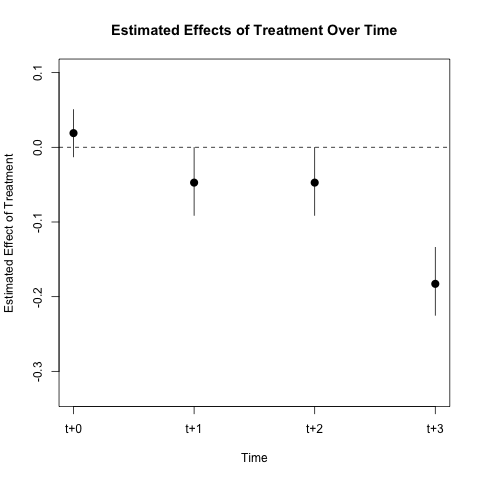
\includegraphics[width=0.9\textwidth]{Chapter1/Figures/acuerdo_gobestatal.png}
       \captionsetup{justification=centering}
       
        
 \textbf{Note:} Figure \ref{fig:matching} produced by propensity score matching that adjust for the treatment and covariate histories during the 5 year periods prior to the treatment. I report 95\% bootstrap confidence intervals clustered at the state level. Covariates include those used to generate Figure \ref{fig:event_study_agreements}. 

\end{figure}   
 
 \clearpage 
\begin{figure}[H] 
\centering
 \caption{Effect of Term Limit Reform on Security Cooperation Agreements signed with the Governor, 2010-2018}
 \label{fig:chaisemarting_agreements}
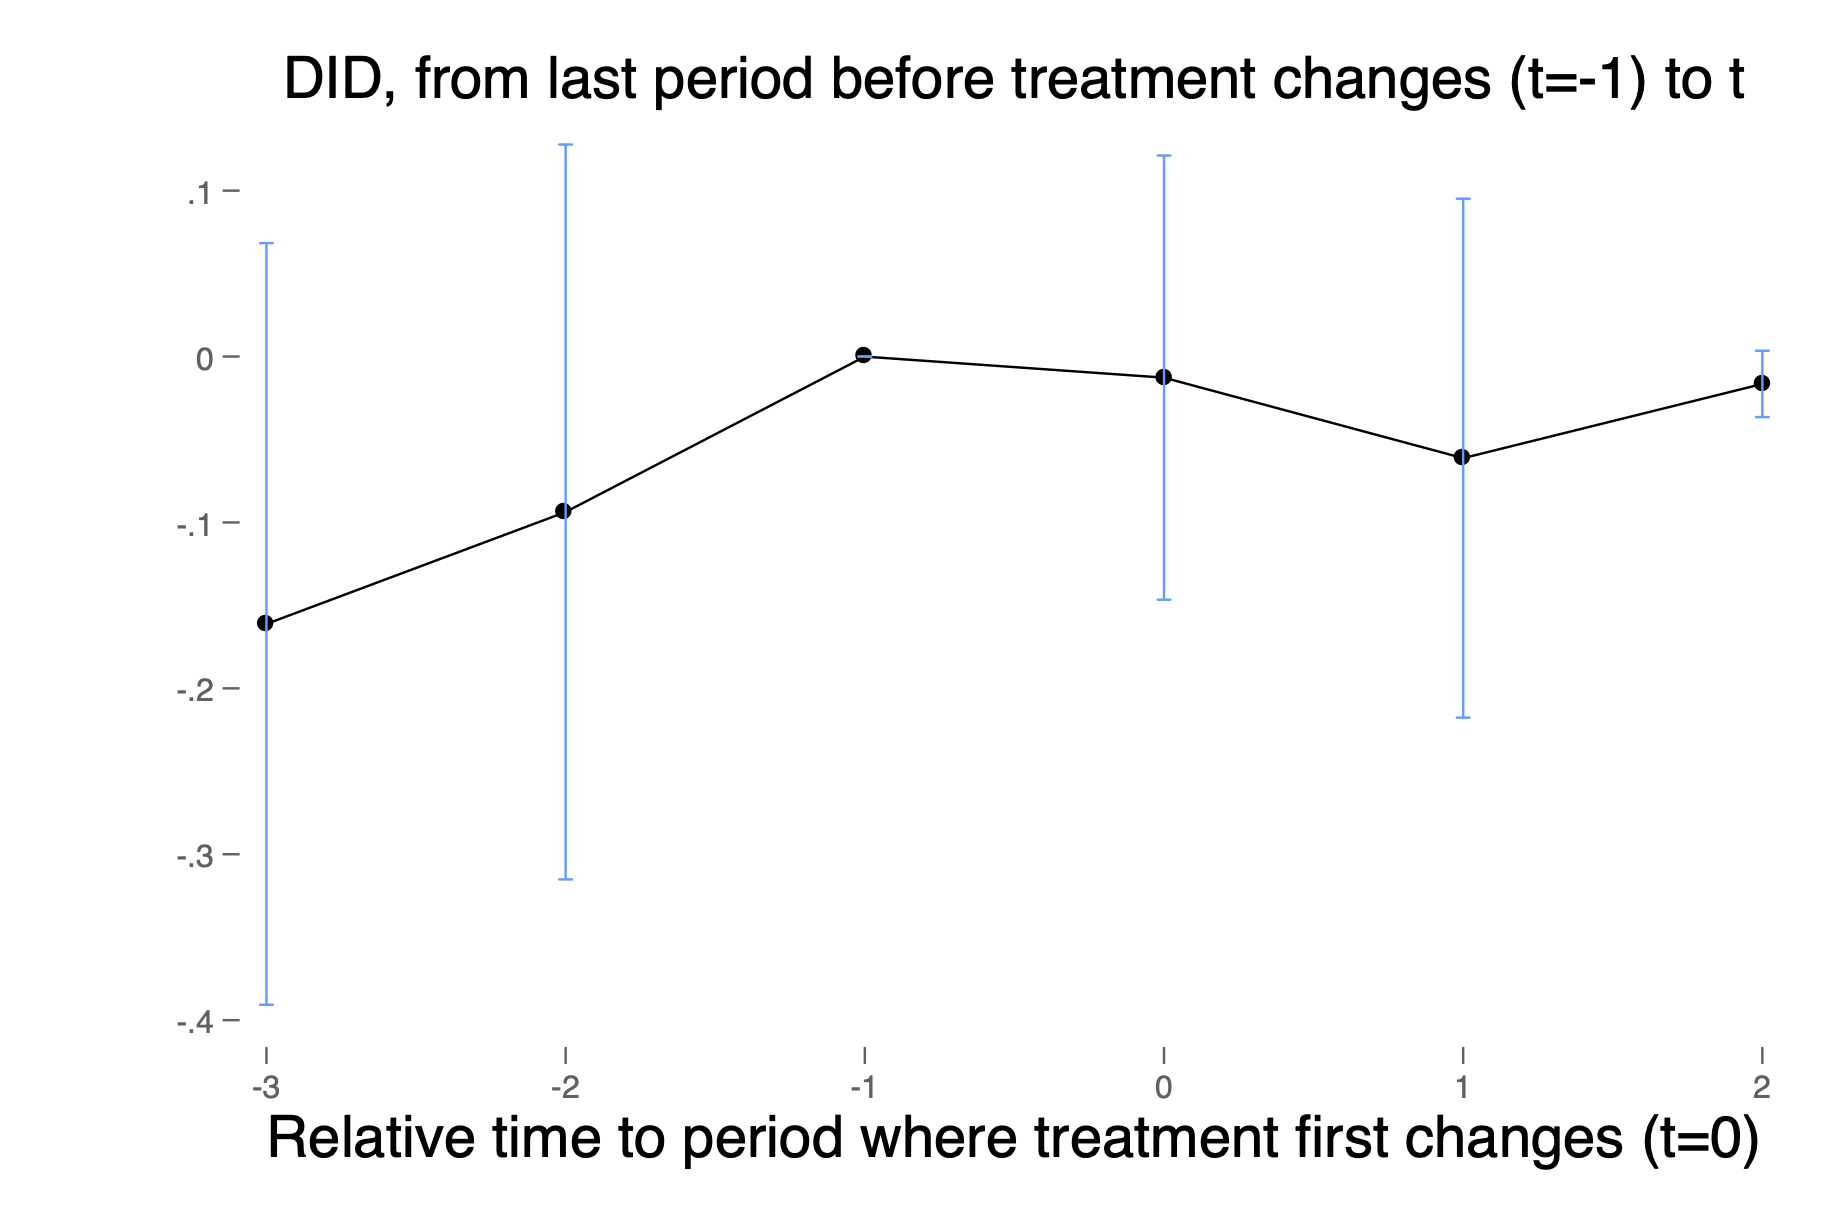
\includegraphics[width=0.9\textwidth]{Chapter1/Figures/chaisemartin_acuerdo_estcom.png}
       \captionsetup{justification=centering}
\end{figure}   

  %\begin{table}[htbp]\def\sym#1{\ifmmode^{#1}\else\(^{#1}\)\fi}
\centering
\caption{Comparison: Security Cooperation Agreements with Governor vs. Other Actors, 2014-2018}
\label{tab:as_comparison_agreements}
\scalebox{1}{
\begin{tabular}{lcc}
\hline \hline
\\ \multicolumn{3}{l}{Dependent variable: Security Cooperation Agreement}\\
& w/ Governor &  w/ Other Political Actors$^a$\\
& \multicolumn{1}{c}{(1)} & \multicolumn{1}{c}{(2)} \\
\cmidrule(lrr){2-2}  \cmidrule(lrr){3-3}\\
\addlinespace
Lag 4 years &         $ 0.0197^{} $ &      $ -0.0326^{} $  \\
& ($ 0.3292$) & ($ 0.0763 $) \\
Lag 3 years &        $ -0.0102^{***} $ &     $ 0.2193^{} $ \\
& ($ 0.0000$) & ($ 0.2702 $) \\
Lag 2 years &        $ 0.1418^{} $ &    $ -0.0648^{} $  \\
& ($ 0.1318$) & ($ 0.0524 $) \\
Reform, time 0 &        $ 0.0064^{} $ &     $ -0.0089^{} $ \\
& ($ 0.0354$) & ($ 0.0069 $) \\
Lead 1 year &         $ -0.2230^{***} $ &       $ -0.2858^{} $ \\
& ($ 0.0435$) & ($ 0.2610 $) \\
Lead 3 years &        $ -0.5921^{***} $ &     $ 0.1665^{} $ \\
& ($ 0.0708$) & ($ 0.1040 $) \\
\addlinespace
Observations       &                  4,382        &           4,382  \\
R-squared        &              0.6434        &           0.5469   \\
Mun. FEs       &     \checkmark         &  \checkmark    \\
Year. FEs       &     \checkmark         &  \checkmark   \\
Controls$^b$   &      \checkmark       &      \checkmark    \\
Cohort weighted   &   \checkmark       &   \checkmark    \\
WILD CI   &          &       \\
Aggregate effect        &              $-0.2696^{***} $$         &            $0.0796^{} $$   \\
SE (aggregate eff.)        &              (0.0339)       &           (0.0491)   \\
\hline \hline
\multicolumn{3}{p{0.7\textwidth}}{\footnotesize{Notes: Coefficients show IW estimators following \citet{abraham_sun_2020}. Two relative time periods (lag 5 and 1) are removed to avoid collinearity problems noted by \citet{abraham_sun_2020}. Standard errors in parentheses are clustered at the state level, with the following significance-level: $^{***}$ 1\%; $^{**}$ 5\%; and $^*$ 10\%, that refer to two-sided t-test with the null hypothesis equal to 0 for each relative time period. $^a$ Refers primarily to the President but could include Governors and mayors from other states or other municipalities from the same state. $^b$ Pretreatment controls include: governor winning margin; party alignment with the President;  party alignment with the Governor; municipal winning margin; logged population; logged organized crime related deaths; and Cartel presence.}} \\
\end{tabular}
}
\end{table}
   
  
  \begin{table}[htbp]\def\sym#1{\ifmmode^{#1}\else\(^{#1}\)\fi}
\centering
\caption{Effect of 2014 Term Limit Reform on the likelihood of signing Security Cooperation Agreements,  by type}
\label{tab:comparison_fed_estatal}
\scalebox{1}{
\begin{tabular}{lcccc}
\hline \hline
\\ \multicolumn{3}{l}{Dependent variable:}\\
& \multicolumn{2}{c}{Security Cooperation Agreement w/ Governor$^{a}$} & \multicolumn{2}{c}{Security Cooperation Agreement w/ Other$^{b}$} \\
& \multicolumn{1}{c}{(1)} & \multicolumn{1}{c}{(2)} & \multicolumn{1}{c}{(3)} & \multicolumn{1}{c}{(4)} \\
\cmidrule(lrr){2-3}  \cmidrule(lrr){4-5}\\
\addlinespace
t-4 &         $ 0.3497^{} $ &         $ 0.0193^{} $ &     $ -0.2763^{} $ &   $ -0.0326^{} $  \\
& ($ 1.8038$) & ($ 0.3316$) & ($ 0.5842$)  & ($ 0.0761 $) \\
t-3 &         $ -0.7355^{} $ &        $ -0.0102^{***} $  &     $ 0.2469^{} $ &     $ 0.2206^{} $ \\
& ($ 37.4159$) & ($ 0.0000$) & ($ 15.0281$) & ($ 0.2702 $) \\
t-2 &         $ 0.3861^{} $ &        $ 0.1420^{} $  &     $ -0.1496^{} $ &    $ -0.0649^{} $  \\
& ($ 0.3279$) & ($ 0.1323$) & ($ 0.1250$) & ($ 0.0524 $) \\
Reform (t=0) &         $ 0.2233^{***} $ &        $ 0.0065^{} $  &     $ -0.0599^{**} $  &     $ -0.0089^{} $ \\
& ($ 0.0581$) & ($ 0.0353$) & ($ 0.0273$) & ($ 0.0070 $) \\
t+1 &         $ -0.2198^{**} $ &         $ -0.2230^{***} $  &     $ 0.1148^{} $ &       $ -0.2845^{} $ \\
& ($ 0.0930$) & ($ 0.0435$) & ($ 0.0904$) & ($ 0.2602 $) \\
t+3 &         $ -0.5915^{***} $ &        $ -0.5921^{***} $ &     $ 0.1660^{*} $  &     $ 0.1665^{} $ \\
& ($ 0.0783$) & ($ 0.0708$) & ($ 0.0953$) & ($ 0.1040 $) \\
\addlinespace
Observations   &                  4,382     &                  4,382  &                  4,382        &           4,382  \\
R-squared      &              0.6433    &              0.6434   &            0.5469        &           0.5469   \\
Mun. FEs       &     \checkmark         &  \checkmark   &     \checkmark         &  \checkmark   \\
Year. FEs       &     \checkmark         &  \checkmark  &     \checkmark         &  \checkmark   \\
Controls$^b$   &      \checkmark       &      \checkmark   &      \checkmark       &      \checkmark   \\
Cohort weighted   &          &   \checkmark   &          &   \checkmark   \\
WILD CI  &     \checkmark         &  \checkmark   &     \checkmark         &  \checkmark   \\
Aggregate effect     &              $-0.213^{***} $$    &        $-0.2696^{***} $$      &            $0.069^{} $$   &       $0.0796^{} $$   \\
SE (aggregate eff.)      &              0.034   &              0.0339    &              0.045       &           0.0491   \\
\hline \hline
\multicolumn{5}{p{1.2\textwidth}}{\footnotesize{Notes: Coefficients in columns (2) and (4) show IW estimators following \citet{abraham_sun_2020}. In those models, two relative time periods (lag 8 and 1) are removed to avoid collinearity problems noted by \citet{abraham_sun_2020}. Standard errors in parentheses are clustered at the state level, with the following significance-level: $^{***}$ 1\%; $^{**}$ 5\%; and $^*$ 10\%, that refer to two-sided t-test with the null hypothesis equal to 0 for each relative time period. $^a$ Refers to security cooperation agreements signed with the governor only. $^b$ Refers to security cooperation agreements signed with other instituions but not the governor. $^c$ State-level controls include governor winning margin in last pre-treatment election and an indicator of whether the governor's party is the same as the federal incumbent party.}} \\
\end{tabular}
}
\end{table}
   
 
 
\def\sym#1{\ifmmode^{#1}\else\(^{#1}\)\fi}
\begin{table}[htbp]\def\sym#1{\ifmmode^{#1}\else\(^{#1}\)\fi}
\centering
\caption{Test on selection on unobservables}
\label{tab:unobservables}
\begin{tabular}{l*{1}{c}}
\hline \hline
&\multicolumn{1}{c}{(1)}         \\
\addlinespace
Fitted value&      0.1312         \\
            &    (0.0780)         \\
\addlinespace
Observations&      10,668         \\
R2          &       0.459         \\
Mun. FE     &      \checkmark               \\
Year FE     &      \checkmark               \\
State Cluster S.E.&     \checkmark                \\
\hline \hline 
\multicolumn{2}{p{0.4\textwidth}}{\footnotesize{Notes: I follow \citet{altonji_etal_2005} to check if unobserved variation is likely to explain the signing of security cooperation agreements with the Governor by mayors. To do so, I regress the treatment (whether the municipality held reelection) on all the available covariates used for Figure \ref{fig:event_study_agreements}.} I then take the fitted value from the regression and use it to predict each outcome, this time including unit and year fixed effects. This test suggests that – under the assumption that observables are representative of unobservables – selection on unobservables is not driving the results.} \\
\end{tabular}
\end{table} 

\clearpage 


\begin{comment}
\begin{figure}[H]
\centering
\caption{Effect of Electoral Reform on Security Cooperation Agreement using non parametric methods\\ -95\% confidence intervals-} 
\label{fig:non_did_agreement}
\begin{center} 
\begin{center} 
	{\textbf Figure A: Generalized Synthetic Control following \citet{xu_2016} }
\end{center}
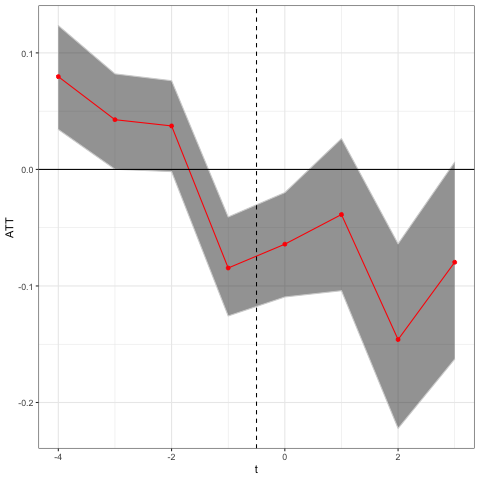
\includegraphics[width=0.55\textwidth]{Chapter1/Figures/gsynth_wcov_acuerdo.png}

\begin{center}
	{\textbf Figure B: Matrix Completion following \citet{Athey, Bayati, Doudchenko, Imbens, and Khosvari}
\end{center}
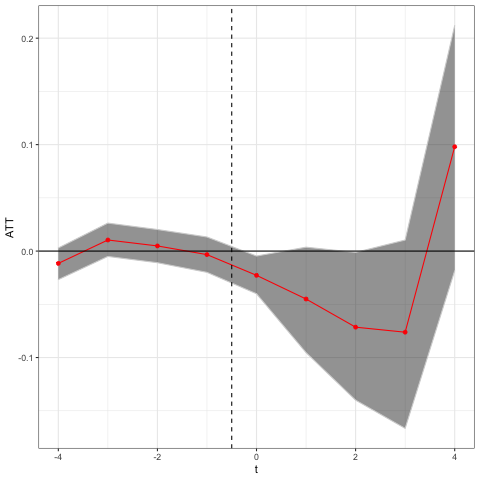
\includegraphics[width=0.55\textwidth]{Chapter1/Figures/matrix_completion.png}
       \captionsetup{justification=centering}
       \\
 %{\textbf Note: 95\% confidence intervals estimated using 1,000 bootstrap replications.} .   
\end{figure}      
\end{comment}


\clearpage

\subsection{Mechanisms}

\begin{figure}[H] 
\centering
 \caption{Effect of 2014 Term Limit Reform on Motives to Sign Security Agreements w/ Governor}
 \label{fig:motives}
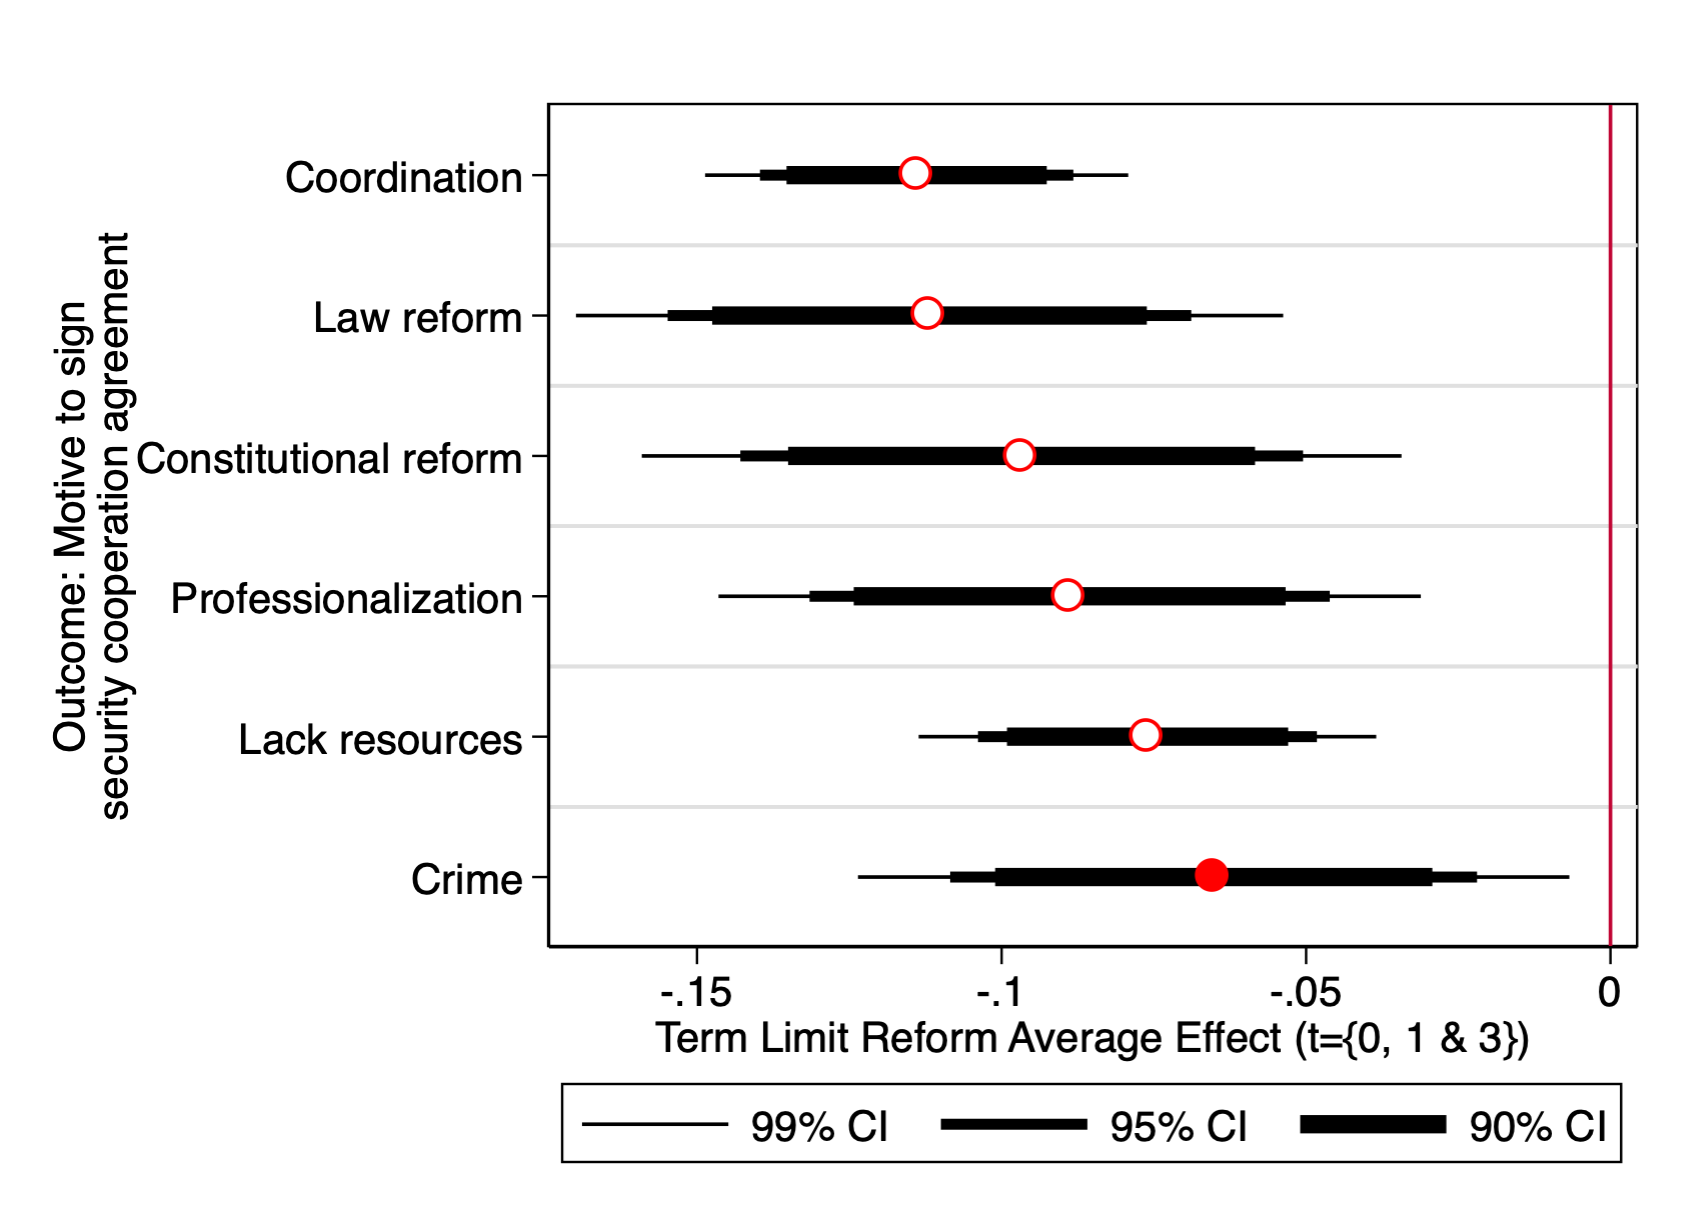
\includegraphics[width=0.9\textwidth]{Chapter1/Figures/motives.png}
       \captionsetup{justification=centering}
\end{figure}   

  \begin{landscape}
\begin{table}[htbp]\def\sym#1{\ifmmode^{#1}\else\(^{#1}\)\fi}
\centering
\caption{Effect of 2014 Term Limit Reform on Motives to Sign Security Agreements w/ Governor}
\label{tab:motives_final}
\scalebox{0.70}{
\begin{tabular}{lcccccc}
\hline \hline
\\ \multicolumn{7}{l}{Dependent variable:}\\
Motive: & Cons. reform  & Law reform & Lack resources & Professionalization & Coordination & Crime \\
& \multicolumn{1}{c}{(1)} & \multicolumn{1}{c}{(2)} & \multicolumn{1}{c}{(3)} & \multicolumn{1}{c}{(4)} & \multicolumn{1}{c}{(5)} & \multicolumn{1}{c}{(6)}  \\
\cmidrule(lrr){2-2}  \cmidrule(lrr){3-3} \cmidrule(lrr){4-4} \cmidrule(lrr){5-5} \cmidrule(lrr){6-6} \cmidrule(lrr){7-7} \\
\addlinespace
t-7 &     $ -0.2350^{***} $ &     $ -0.2581^{**} $ & $ -0.0955^{*} $ & $ -0.2000^{***} $  &     $ -0.1570^{*} $   &     $ -0.1538^{} $ \\
&     ($0.0407$) &     ($0.1175$) & ($0.0484$)& ($ 0.0671$)  &    ($0.0844$)   &   ($0.1078$) \\
t-6 &     $ -0.0758^{***} $ &     $ -0.0876^{***} $ &  $ -0.0615^{***} $ &  $ -0.0647^{} $  &     $ -0.0827^{**} $ &     $ -0.0369^{} $ \\
&     ($0.0176$) &     ($0.0199$) & ($0.0162$)& ($ 0.0585$)  &    ($0.0346$)   &   ($0.0265$) \\
t-5 &     $ 0.0223^{} $ &     $ -0.0405^{} $ &  $ 0.0574^{} $ &  $ 0.0580^{} $ &     $ -0.0106^{} $  &     $ 0.0427^{} $ \\
&     ($0.0591$) &     ($0.0583$) & ($0.0481$)& ($ 0.0750$)  &    ($0.0709$)   &   ($0.0445$) \\
t-4 &     $ 0.0167^{} $ &     $ -0.0832^{} $ &   $ 0.1207^{} $ &   $ 0.0649^{} $  &     $ -0.1313^{} $ &     $ 0.0346^{} $ \\
&     ($0.0987$) &     ($0.0842$) & ($0.0854$)& ($ 0.1053$)  &    ($0.2085$)   &   ($0.1173$) \\
t-3 &     $ -0.0385^{} $ &     $ -0.0160^{} $ &   $ 0.0727^{} $ &   $ 0.0802^{} $  &     $ 0.0403^{} $ &     $ 0.0734^{} $ \\
&     ($0.1052$) &     ($0.0840$) & ($0.1002$)& ($ 0.0738$)  &    ($0.1662$)   &   ($0.1061$) \\
t-2 &     $ -0.1162^{} $ &     $ -0.0914^{} $ &  $ 0.0228^{} $  &  $ -0.0822^{} $  &     $ -0.2796^{*} $ &     $ -0.0753^{} $ \\
&     ($0.1012$) &     ($0.0917$) & ($0.0640$)& ($ 0.1195$)  &    ($0.1379$)   &   ($0.0667$) \\
Reform (t=0) &     $ 0.0457^{} $ &     $ 0.0292^{} $ &   $ 0.0214^{} $   &   $ 0.0282^{} $  &     $ 0.0233^{} $ &     $ 0.0272^{*} $ \\
&     ($0.0278$) &     ($0.0183$) & ($0.0179$)& ($ 0.0201$)  &    ($0.0209$)   &   ($0.0146$) \\
t+1 &     $ -0.0906^{***} $ &     $ -0.1071^{***} $ &    $ -0.0935^{***} $ &    $ -0.0935^{***} $ &     $ -0.1215^{***} $ &     $ -0.0735^{***} $  \\
&     ($0.0164$) &     ($0.0182$) & ($0.0106$)& ($ 0.0160$)  &    ($0.0291$)   &   ($0.0121$) \\
t+3 &     $ -0.2452^{***} $ &     $ -0.2576^{***} $ &   $ -0.1560^{***} $  &   $ -0.2011^{***} $ &     $ -0.2436^{***} $ &     $ -0.1492^{***} $ \\
&     ($0.0535$) &     ($0.0484$) & ($0.0350$)& ($ 0.0463$)  &    ($0.0431$)   &   ($0.0527$) \\
\\
\addlinespace
Observations       &              9,725    &              9,725    &           9,725      &           9,725  &              9,725    &              9,725     \\
R-squared        &          0.2974 &          0.3021    &    0.2617       &           0.2722 &          0.2865 &          0.2594      \\
Mun. FEs      &     \checkmark         &  \checkmark   &     \checkmark         &  \checkmark  &     \checkmark         &  \checkmark   &     \checkmark         &  \checkmark   \\
Year. FEs    &     \checkmark         &  \checkmark   &     \checkmark         &  \checkmark &     \checkmark         &  \checkmark   &     \checkmark         &  \checkmark   \\
Controls$^b$  &    \checkmark     &       \checkmark  &    \checkmark      &   \checkmark &    \checkmark     &       \checkmark  &    \checkmark      &   \checkmark     \\
Cohort weighted  &   \checkmark      &       \checkmark  &   \checkmark       &   \checkmark  &   \checkmark      &       \checkmark  &   \checkmark       &   \checkmark    \\
Reform aggregate effect         & $-0.0967^{***} $$      & $-0.1118^{***} $$    & $-0.0760^{***} $$      & $-0.0888^{***} $$     & $-0.1139^{***} $$      & $-0.0652^{***} $$     \\
SE       & (0.0225)  & (0.0210) & (0.0136)  & (0.0208)  & (0.0125)  & (0.0211)   \\
\hline \hline
\multicolumn{7}{p{1.2\textwidth}}{\footnotesize{Notes: Coefficients show IW estimators following \citet{abraham_sun_2020}. Two relative time periods (lag 8 and 1) are removed to avoid collinearity problems noted by \citet{abraham_sun_2020}. Standard errors in parentheses are clustered at the state level for estimates in saturaded model. Significance-level: $^{***}$ 1\%; $^{**}$ 5\%; and $^*$ 10\%, that refer to two-sided t-test with the null hypothesis equal to 0 for each relative time period. $^a$ Even columns with outcomes with missing values where replaced by zeros assuming no activity was registered. $^b$ State-level controls include governor winning margin in last pre-treatment election and an indicator of whether the governor's party is the same as the federal incumbent party.}} \\
\end{tabular}
}
\end{table}
\end{landscape}
   

   %\begin{landscape}
\begin{table}[htbp]\def\sym#1{\ifmmode^{#1}\else\(^{#1}\)\fi}
\centering
\caption{Effect of 2014 Term Limit Reform on Motives to Sign Security Agreements w/ Governor}
\label{tab:motives_average_final}
\scalebox{0.70}{
\begin{tabular}{lcccccc}
\hline \hline
\\ \multicolumn{7}{l}{Dependent variable:}\\
Motive: & Cons. reform  & Law reform & Lack resources & Professionalization & Coordination & Crime \\
& \multicolumn{1}{c}{(1)} & \multicolumn{1}{c}{(2)} & \multicolumn{1}{c}{(3)} & \multicolumn{1}{c}{(4)} & \multicolumn{1}{c}{(5)} & \multicolumn{1}{c}{(6)}  \\
\cmidrule(lrr){2-2}  \cmidrule(lrr){3-3} \cmidrule(lrr){4-4} \cmidrule(lrr){5-5} \cmidrule(lrr){6-6} \cmidrule(lrr){7-7} \\
\addlinespace
Reform average effect         & $-0.0967^{***} $$      & $-0.1118^{***} $$     & $-0.0760^{***} $$        & $-0.0888^{***} $$       & $-0.1139^{***} $$        & $-0.0652^{***} $$       \\
& (0.0225)  & (0.0210) & (0.0136)  & (0.0208)  & (0.0125)  & (0.0211)   \\
\\
\addlinespace
Observations       &              9,725    &              9,725    &           9,725      &           9,725  &              9,725    &              9,725    \\
R-squared        &          0.2974 &          0.3021    &    0.2617       &           0.2722 &          0.2865 &          0.2594   \\
Mun. FEs      &     \checkmark         &  \checkmark   &     \checkmark         &  \checkmark  &     \checkmark         &  \checkmark   &     \checkmark         &  \checkmark   \\
Year. FEs    &     \checkmark         &  \checkmark   &     \checkmark         &  \checkmark &     \checkmark         &  \checkmark   &     \checkmark         &  \checkmark   \\
Controls$^b$  &    \checkmark     &       \checkmark  &    \checkmark      &   \checkmark &    \checkmark     &       \checkmark  &    \checkmark      &   \checkmark     \\
Cohort weighted  &   \checkmark      &       \checkmark  &   \checkmark       &   \checkmark  &   \checkmark      &       \checkmark  &   \checkmark       &   \checkmark    \\
Parallel trend holds &   \checkmark      &       \checkmark  &   \checkmark       &   \checkmark  &   \checkmark      &       \checkmark  &   \checkmark       &   \checkmark    \\
\hline \hline
\multicolumn{7}{p{1.2\textwidth}}{\footnotesize{Notes: Coefficients show IW estimators following \citet{abraham_sun_2020}. Two relative time periods (lag 8 and 1) are removed to avoid collinearity problems noted by \citet{abraham_sun_2020}. Standard errors in parentheses are clustered at the state level for estimates in saturaded model. Significance-level: $^{***}$ 1\%; $^{**}$ 5\%; and $^*$ 10\%, that refer to two-sided t-test with the null hypothesis equal to 0 for each relative time period. $^a$ Even columns with outcomes with missing values where replaced by zeros assuming no activity was registered. $^b$ State-level controls include governor winning margin in last pre-treatment election and an indicator of whether the governor's party is the same as the federal incumbent party.}} \\
\end{tabular}
}
\end{table}
\end{landscape}
  
   
   
      
\begin{landscape}
\begin{table}[htbp]\def\sym#1{\ifmmode^{#1}\else\(^{#1}\)\fi}
\centering
\caption{Effect of 2014 Term Limit Reform on Services Delegated to the Governor}
\label{tab:services}
\scalebox{0.70}{
\begin{tabular}{lcccccccc}
\hline \hline
\\ \multicolumn{9}{l}{Dependent variable:}\\
Service delegated: & Public security  & Traffic & Prevention & Training  & Technology & Research & Inteligence & Unify procedures \\
& \multicolumn{1}{c}{(1)} & \multicolumn{1}{c}{(2)} & \multicolumn{1}{c}{(3)} & \multicolumn{1}{c}{(4)} & \multicolumn{1}{c}{(5)} & \multicolumn{1}{c}{(6)} & \multicolumn{1}{c}{(7)} & \multicolumn{1}{c}{(8)} \\
\cmidrule(lrr){2-2}  \cmidrule(lrr){3-3} \cmidrule(lrr){4-4} \cmidrule(lrr){5-5} \cmidrule(lrr){6-6} \cmidrule(lrr){7-7} \cmidrule(lrr){8-8} \cmidrule(lrr){9-9} \\
\addlinespace
t-2 &     $ -0.0244^{} $ &     $ -0.0441^{} $ &  $ -0.0598^{***} $  &  $ -0.0565^{***} $  &     $ -0.0567^{***} $ &     $ -0.0596^{***} $ & $ -0.0596^{***} $ & $ -0.0506^{***} $   \\
&     ($0.1046$) &     ($0.0818$) & ($0.0021$)& ($ 0.0012$)  &    ($0.0016$)   &   ($0.0017$) \\
Reform (t=0) &     $ 0.0702^{} $ &     $ 0.0256^{} $ &   $ 0.0175^{} $   &   $ 0.0214^{} $  &     $ 0.0194^{} $ &     $ 0.0194^{} $ & $ 0.0204^{} $ & $ 0.0233^{} $   \\
&     ($0.0436$) &     ($0.0369$) & ($0.0137$)& ($ 0.0142$)  &    ($0.0126$)   &   ($0.0138$) \\
t+1 &     $ -0.0947^{*} $ &     $ -0.0259^{*} $ &    $ 0.0106^{} $ &    $ 0.0053^{} $ &     $ 0.0047^{} $ &     $ 0.0024^{} $  & $ 0.0018^{} $ & $ 0.0053^{} $   \\
&     ($0.0509$) &     ($0.0147$) & ($0.0198$)& ($ 0.0193$)  &    ($0.0197$)   &   ($0.0201$) \\
t+3 &     $ -0.2847^{***} $ &     $ 0.0000^{} $  \\
&     ($0.0430$) &     ($0.0000$)  \\
\\
\addlinespace
Observations       &              4,865    &              4,865    &           3,244      &           3,244  &              3,244    &              3,244  &              3,244    &              6,481   \\
R-squared        &          0.4234 &          0.3703    &    0.5567       &           0.5477 &          0.5409 &          0.5473     &        0.5467    &        0.4894   \\
Mun. FEs      &     \checkmark         &  \checkmark   &     \checkmark         &  \checkmark  &     \checkmark         &  \checkmark   &     \checkmark         &  \checkmark   \\
Year. FEs    &     \checkmark         &  \checkmark   &     \checkmark         &  \checkmark &     \checkmark         &  \checkmark   &     \checkmark         &  \checkmark   \\
Controls$^b$  &    \checkmark     &       \checkmark  &    \checkmark      &   \checkmark &    \checkmark     &       \checkmark  &    \checkmark      &   \checkmark     \\
Cohort weighted  &   \checkmark      &       \checkmark  &   \checkmark       &   \checkmark  &   \checkmark      &       \checkmark  &   \checkmark       &   \checkmark    \\
Reform average effect         & $-0.1031^{***} $$      & $-0.0242^{} $$     & $0.0094^{} $$        & $0.0133^{} $$       & $0.0121^{} $$        & $0.0109^{} $$    & $0.0111^{} $$      & $0.0143^{} $$     \\
SE (average effect)      & (0.0225)  & (0.0162) & (0.0080)  & (0.0120)  & (0.0117)  & (0.0122)    & (0.0123)  & (0.0114)   \\
\hline \hline
\multicolumn{9}{p{1.5\textwidth}}{\footnotesize{Notes: Coefficients show IW estimators following \citet{abraham_sun_2020}. Two relative time periods (lag 8 and 1) are removed to avoid collinearity problems noted by \citet{abraham_sun_2020}. Standard errors in parentheses are clustered at the state level for estimates in saturaded model. Significance-level: $^{***}$ 1\%; $^{**}$ 5\%; and $^*$ 10\%, that refer to two-sided t-test with the null hypothesis equal to 0 for each relative time period. $^a$ Even columns with outcomes with missing values where replaced by zeros assuming no activity was registered. $^b$ State-level controls include governor winning margin in last pre-treatment election and an indicator of whether the governor's party is the same as the federal incumbent party.}} \\
\end{tabular}
}
\end{table}
\end{landscape}
   
%\begin{landscape}
\begin{table}[htbp]\def\sym#1{\ifmmode^{#1}\else\(^{#1}\)\fi}
\centering
\caption{Effect of 2014 Term Limit Reform on Services Delegated to the Governor}
\label{tab:services_average}
\scalebox{0.70}{
\begin{tabular}{lcccccccc}
\hline \hline
\\ \multicolumn{9}{l}{Dependent variable:}\\
Service delegated: & Public security  & Traffic & Prevention & Training  & Technology & Research & Inteligence & Unify procedures \\
& \multicolumn{1}{c}{(1)} & \multicolumn{1}{c}{(2)} & \multicolumn{1}{c}{(3)} & \multicolumn{1}{c}{(4)} & \multicolumn{1}{c}{(5)} & \multicolumn{1}{c}{(6)} & \multicolumn{1}{c}{(7)} & \multicolumn{1}{c}{(8)} \\
\cmidrule(lrr){2-2}  \cmidrule(lrr){3-3} \cmidrule(lrr){4-4} \cmidrule(lrr){5-5} \cmidrule(lrr){6-6} \cmidrule(lrr){7-7} \cmidrule(lrr){8-8} \cmidrule(lrr){9-9} \\
\addlinespace
Reform average effect         & $0.0149^{*} $$      & $0.0579^{***} $$     & $0.0426^{***} $$        & $0.0034^{} $$       & $-0.0345^{***} $$        & $-0.0819^{***} $$    & $0.0092^{} $$      & $0.0056^{} $$     \\
SE       & (0.0079)  & (0.0099) & (0.0046)  & (0.0048)  & (0.0103)  & (0.0085)    & (0.0063)  & (0.0034)   \\
\addlinespace
Observations       &             11,353    &             11,353    &          11,353      &          11,353  &             11,353    &             11,353  &             11,353    &             11,353   \\
R-squared        &          0.8662 &          0.8556    &    0.9239       &           0.8767 &          0.8548 &          0.8954     &        0.8557    &        0.7008   \\
Mun. FEs      &     \checkmark         &  \checkmark   &     \checkmark         &  \checkmark  &     \checkmark         &  \checkmark   &     \checkmark         &  \checkmark   \\
Year. FEs    &     \checkmark         &  \checkmark   &     \checkmark         &  \checkmark &     \checkmark         &  \checkmark   &     \checkmark         &  \checkmark   \\
Controls$^b$  &    \checkmark     &       \checkmark  &    \checkmark      &   \checkmark &    \checkmark     &       \checkmark  &    \checkmark      &   \checkmark     \\
Cohort weighted  &   \checkmark      &       \checkmark  &   \checkmark       &   \checkmark  &   \checkmark      &       \checkmark  &   \checkmark       &   \checkmark    \\
Parallel trend holds &   \checkmark      &       \checkmark  &          &     &         &       &          &       \\
\hline \hline
\multicolumn{9}{p{1.5\textwidth}}{\footnotesize{Notes: Coefficients show IW estimators following \citet{abraham_sun_2020}. Two relative time periods (lag 8 and 1) are removed to avoid collinearity problems noted by \citet{abraham_sun_2020}. Standard errors in parentheses are clustered at the state level for estimates in saturaded model. Significance-level: $^{***}$ 1\%; $^{**}$ 5\%; and $^*$ 10\%, that refer to two-sided t-test with the null hypothesis equal to 0 for each relative time period. $^a$ Even columns with outcomes with missing values where replaced by zeros assuming no activity was registered. $^b$ State-level controls include governor winning margin in last pre-treatment election and an indicator of whether the governor's party is the same as the federal incumbent party.}} \\
\end{tabular}
}
\end{table}
\end{landscape}
   

\begin{landscape}
\begin{table}[htbp]\def\sym#1{\ifmmode^{#1}\else\(^{#1}\)\fi}
\centering
\caption{Effect of 2014 Term Limit Reform on Services Delegated to the Governor}
\label{tab:interaction_alignment}
\scalebox{0.70}{
\begin{tabular}{lccc}
\hline \hline
\\ \multicolumn{4}{l}{Dependent variable: Signing Security Cooperation Agreement w/ Governor}\\
Alignment: & w/ President  & w/ Governor  & w/ Governor from PRI \\
& \multicolumn{1}{c}{(1)} & \multicolumn{1}{c}{(2)} & \multicolumn{1}{c}{(3)} \\
\cmidrule(lrr){2-2}  \cmidrule(lrr){3-3} \cmidrule(lrr){4-4} \\
\addlinespace
t-7 &     $ -0.2383^{*} $ &     $ -0.0191^{*} $ &  $ 0.0000^{} $ \\
&     ($0.1348$) &     ($0.0108$) & ($0.0000$) \\
t-6 &     $ -0.0807^{} $ &     $ 0.0199^{} $ &  $ -0.0430^{} $  \\
&     ($0.0873$) &     ($0.0499$) & ($0.0467$) \\
t-5 &     $ -0.1186^{} $ &     $ -0.2028^{**} $ &  $ -0.2406^{**} $  \\
&     ($0.1046$) &     ($0.0924$) & ($0.0922$) \\
t-4 &     $ 0.0665^{} $ &     $ -0.0784^{} $ &  $ -0.1077^{} $  \\
&     ($0.1483$) &     ($0.1203$) & ($0.1236$) \\
t-3 &     $ 0.3395^{**} $ &     $ 0.2569^{***} $ &  $ 0.2303^{***} $  \\
&     ($0.1651$) &     ($0.0720$) & ($0.0702$) \\
t-2 &     $ 0.0027^{} $ &     $ -0.0253^{} $ &  $ 0.0976^{} $  \\
&     ($0.1572$) &     ($0.1182$) & ($0.1471$) \\
Reform (t=0) &     $ -0.1686^{} $ &     $ -0.2236^{} $ &   $ 0.1790^{} $   \\
&     ($0.1877$) &     ($0.1316$) & ($0.1258$) \\
t+1 &     $ -0.2169^{} $ &     $ -0.5692^{**} $ &    $ -0.0199^{} $ \\
&     ($0.1884$) &     ($0.2119$) & ($0.1549$) \\
t+2 &     $ -0.1125^{} $ &     $ -0.5020^{*} $  &     $ -0.4753^{*} $ \\
&     ($0.2496$) &     ($0.2690$)  & ($0.2741$) \\
t+3 &     $ -0.2197^{} $ &     $ -0.3562^{} $  &     $ -0.3876^{} $ \\
&     ($0.2241$) &     ($0.3827$)  & ($0.3818$) \\
\\
\addlinespace
Observations       &             12,173    &             12,173    &          12,173    \\
R-squared        &          0.4555 &          0.4566    &    0.4541    \\
Mun. FEs      &     \checkmark         &  \checkmark   &     \checkmark    \\
Year. FEs    &     \checkmark         &  \checkmark   &     \checkmark    \\
Controls$^b$  &    \checkmark     &       \checkmark  &    \checkmark   \\
Cohort weighted  &   \checkmark      &       \checkmark  &   \checkmark    \\
Reform average effect         & $-0.1376^{} $$      & $-0.1538^{*} $$     & $-0.0551^{} $$     \\
SE (average effect)      & (0.1313)  & (0.0906) & (0.0652) \\
\hline \hline
\multicolumn{4}{p{1.5\textwidth}}{\footnotesize{Notes: Coefficients show IW estimators following \citet{abraham_sun_2020}. Two relative time periods (lag 8 and 1) are removed to avoid collinearity problems noted by \citet{abraham_sun_2020}. Standard errors in parentheses are clustered at the state level for estimates in saturaded model. Significance-level: $^{***}$ 1\%; $^{**}$ 5\%; and $^*$ 10\%, that refer to two-sided t-test with the null hypothesis equal to 0 for each relative time period. $^a$ Even columns with outcomes with missing values where replaced by zeros assuming no activity was registered. $^b$ State-level controls include governor winning margin in last pre-treatment election and an indicator of whether the governor's party is the same as the federal incumbent party.}} \\
\end{tabular}
}
\end{table}
\end{landscape}
   
%\begin{landscape}
\begin{table}[htbp]\def\sym#1{\ifmmode^{#1}\else\(^{#1}\)\fi}
\centering
\caption{Effect of 2014 Term Limit Reform on Services Delegated to the Governor}
\label{tab:interaction_alignment_average}
\scalebox{0.70}{
\begin{tabular}{lccc}
\hline \hline
\\ \multicolumn{4}{l}{Dependent variable: Signing Security Cooperation Agreement w/ Governor}\\
Alignment: & w/ President  & w/ Governor  & w/ Governor from PRI \\
& \multicolumn{1}{c}{(1)} & \multicolumn{1}{c}{(2)} & \multicolumn{1}{c}{(3)} \\
\cmidrule(lrr){2-2}  \cmidrule(lrr){3-3} \cmidrule(lrr){4-4} \\
\addlinespace
Reform average effect         & $-0.1376^{} $$      & $-0.1538^{*} $$     & $-0.0551^{} $$     \\
& (0.1313)  & (0.0906) & (0.0652) \\
\\
\addlinespace
Observations       &             12,173    &             12,173    &          12,173    \\
R-squared        &          0.4555 &          0.4566    &    0.4541    \\
Mun. FEs      &     \checkmark         &  \checkmark   &     \checkmark    \\
Year. FEs    &     \checkmark         &  \checkmark   &     \checkmark    \\
Controls$^b$  &    \checkmark     &       \checkmark  &    \checkmark   \\
Cohort weighted  &   \checkmark      &       \checkmark  &   \checkmark    \\
\hline \hline
\multicolumn{4}{p{1.5\textwidth}}{\footnotesize{Notes: Coefficients show IW estimators following \citet{abraham_sun_2020}. Two relative time periods (lag 8 and 1) are removed to avoid collinearity problems noted by \citet{abraham_sun_2020}. Standard errors in parentheses are clustered at the state level for estimates in saturaded model. Significance-level: $^{***}$ 1\%; $^{**}$ 5\%; and $^*$ 10\%, that refer to two-sided t-test with the null hypothesis equal to 0 for each relative time period. $^a$ Even columns with outcomes with missing values where replaced by zeros assuming no activity was registered. $^b$ State-level controls include governor winning margin in last pre-treatment election and an indicator of whether the governor's party is the same as the federal incumbent party.}} \\
\end{tabular}
}
\end{table}
\end{landscape}
   

              
\begin{landscape}
\begin{table}[htbp]\def\sym#1{\ifmmode^{#1}\else\(^{#1}\)\fi}
\centering
\caption{Reform interaction with citizens' preferences}
\label{tab:interaction_trust}
\scalebox{0.70}{
\begin{tabular}{lcccccccc}
\hline \hline
\\ \multicolumn{9}{l}{Dependent variable: Signing Security Cooperation Agreement w/ Governor}\\
Jurisdiction: & \multicolumn{2}{c}{Municipal} & \multicolumn{2}{c}{State} & \multicolumn{4}{c}{Federal} \\
Trust in Police Force: & Traffic  & Preventive  & State Police & State Attorney Police & Federal Police & Ministerial Police & Army & Marines \\
& \multicolumn{1}{c}{(1)} & \multicolumn{1}{c}{(2)} & \multicolumn{1}{c}{(3)} & \multicolumn{1}{c}{(4)} & \multicolumn{1}{c}{(5)} & \multicolumn{1}{c}{(6)} & \multicolumn{1}{c}{(7)} & \multicolumn{1}{c}{(8)} \\
\cmidrule(lrr){2-2}  \cmidrule(lrr){3-3} \cmidrule(lrr){4-4} \cmidrule(lrr){5-5} \cmidrule(lrr){6-6} \cmidrule(lrr){7-7} \cmidrule(lrr){8-8} \cmidrule(lrr){9-9} \\
\addlinespace
t-7 &     $ 0.1781^{} $ &     $ 0.0000^{} $ &  $ 0.1737^{} $  &  $ 0.1269^{} $  &     $ 0.0908^{} $ &     $ 0.1162^{} $ & $ 0.1093^{*} $ & $ 0.0788^{} $   \\
&     ($0.1657$) &     ($0.0000$) & ($0.1372$)& ($ 0.1137$)  &    ($0.0736$)   &   ($0.0858$) &    ($0.0638$)   &   ($0.0557$) \\
t-6 &     $ -0.0459^{} $ &     $ -0.0601^{} $ &  $ -0.0415^{} $  &  $ -0.0566^{} $  &     $ 0.0056^{} $ &     $ -0.0538^{} $ & $ 0.0234^{} $ & $ 0.0038^{} $   \\
&     ($0.0801$) &     ($0.0481$) & ($0.0539$)& ($ 0.0457$)  &    ($0.0390$)   &   ($0.0379$) &    ($0.0413$)   &   ($0.0413$) \\
t-5 &     $ -0.8924^{***} $ &     $ -0.2958^{} $ &  $ -0.7754^{} $  &  $ -1.3248^{} $  &     $ -0.8583^{**} $ &     $ -1.3845^{***} $ & $ -0.6699^{**} $ & $ -0.5789^{} $   \\
&     ($0.2538$) &     ($0.2471$) & ($0.6290$)& ($ 0.9127$)  &    ($0.3310$)   &   ($0.2852$) &    ($0.3135$)   &   ($0.3456$) \\
t-4 &     $ -0.8378^{} $ &     $ -0.4847^{} $ &  $ -0.8334^{} $  &  $ -1.8134^{} $  &     $ -1.0907^{} $ &     $ -1.2390^{} $ & $ -0.3788^{} $ & $ -0.4918^{} $   \\
&     ($0.7686$) &     ($0.7828$) & ($0.7594$)& ($ 1.3211$)  &    ($0.7492$)   &   ($1.0418$) &    ($0.5581$)   &   ($0.6697$) \\
t-3 &     $ -0.0583^{} $ &     $ -0.2255^{} $ &  $ -0.4855^{} $  &  $ -1.8474^{} $  &     $ -0.6963^{} $ &     $ -0.8293^{} $ & $ 0.1189^{} $ & $ -0.1128^{} $   \\
&     ($0.8134$) &     ($0.8597$) & ($0.7510$)& ($ 1.3390$)  &    ($0.8562$)   &   ($1.1144$) &    ($0.6286$)   &   ($0.7221$) \\
t-2 &     $ 0.0349^{} $ &     $ -0.2669^{} $ &  $ -0.2886^{} $  &  $ -0.6193^{} $  &     $ -0.6132^{} $ &     $ -0.3460^{} $ & $ -0.4240^{} $ & $ -0.4018^{} $   \\
&     ($0.5384$) &     ($0.5922$) & ($0.4176$)& ($ 0.8964$)  &    ($0.4795$)   &   ($0.7851$) &    ($0.3186$)   &   ($0.4479$) \\
Reform (t=0) &     $ -0.4445^{} $ &     $ 0.1161^{} $ &   $ -0.5433^{} $   &   $ -0.3590^{} $  &     $ -1.2945^{**} $ &     $ -0.8582^{} $ & $ -0.4517^{} $ & $ -0.8450^{} $   \\
&     ($0.4490$) &     ($0.4974$) & ($0.4116$)& ($ 1.1629$)  &    ($0.5674$)   &   ($0.7679$) &    ($0.4624$)   &   ($0.5361$) \\
t+1 &     $ -0.9837^{} $ &     $ -0.2187^{} $ &    $ -1.3877^{**} $ &    $ -1.3448^{} $ &     $ -2.4944^{***} $ &     $ -1.8551^{*} $  & $ -1.5411^{**} $ & $ -1.8923^{**} $   \\
&     ($0.5947$) &     ($0.5769$) & ($0.6053$)& ($ 1.4393$)  &    ($0.7475$)   &   ($0.9450$) &    ($0.6971$)   &   ($0.6934$) \\
t+2 &     $ -1.8509^{***} $ &     $ -1.6314^{**} $ &    $ -1.9022^{**} $ &    $ -4.0615^{***} $ &     $ -2.2753^{***} $ &     $ -3.3031^{***} $  & $ -1.2009^{} $ & $ -1.8294^{**} $   \\
&     ($0.5939$) &     ($0.6872$) & ($0.8555$)& ($ 1.1352$)  &    ($0.7941$)   &   ($0.6820$) &    ($0.7654$)   &   ($0.6810$) \\
t+3 &     $ -0.1382^{} $ &     $ -1.5280^{} $ &    $ -0.9653^{} $ &    $ -1.9755^{*} $ &     $ -0.9980^{} $ &     $ -1.1886^{} $  & $ 0.0385^{} $ & $ -0.9525^{} $   \\
&     ($1.1166$) &     ($1.1456$) & ($0.7908$)& ($ 1.0802$)  &    ($1.4571$)   &   ($1.2863$) &    ($1.1601$)   &   ($1.1245$) \\
\\
\addlinespace
Observations       &             12,173    &             12,173    &          12,173      &          12,173  &             12,173    &             12,173  &             12,173    &             12,173   \\
R-squared        &          0.4666 &          0.4641    &    0.4675       &           0.4673 &          0.4642 &          0.4719     &        0.4666    &        0.4666   \\
Mun. FEs      &     \checkmark         &  \checkmark   &     \checkmark         &  \checkmark  &     \checkmark         &  \checkmark   &     \checkmark         &  \checkmark   \\
Year. FEs    &     \checkmark         &  \checkmark   &     \checkmark         &  \checkmark &     \checkmark         &  \checkmark   &     \checkmark         &  \checkmark   \\
Controls$^b$  &    \checkmark     &       \checkmark  &    \checkmark      &   \checkmark &    \checkmark     &       \checkmark  &    \checkmark      &   \checkmark     \\
Cohort weighted  &   \checkmark      &       \checkmark  &   \checkmark       &   \checkmark  &   \checkmark      &       \checkmark  &   \checkmark       &   \checkmark    \\
Reform average effect         & $-0.1400^{} $$      & $-0.2053^{} $$     & $-0.3431^{**} $$        & $-0.2984^{**} $$       & $-0.5739^{**} $$        & $-0.2614^{**} $$    & $-0.4636^{} $$      & $-0.4837^{*} $$     \\
SE (average effect)      & (0.0944)  & (0.1633) & (0.1594)  & (0.1455)  & (0.2673)  & (0.1107)    & (0.4248)  & (0.2374)   \\
\hline \hline
\multicolumn{9}{p{1.8\textwidth}}{\footnotesize{Notes: Coefficients show IW estimators following \citet{abraham_sun_2020}. Two relative time periods (lag 8 and 1) are removed to avoid collinearity problems noted by \citet{abraham_sun_2020}. Standard errors in parentheses are clustered at the state level, with the following significance-level: $^{***}$ 1\%; $^{**}$ 5\%; and $^*$ 10\%, that refer to two-sided t-test with the null hypothesis equal to 0 for each relative time period. $^a$ Refers to security cooperation agreements signed with the Governor. $^b$ Pretreatment controls include: governor winning margin; party alignment with the President;  party alignment with the Governor; municipal winning margin; logged population; logged organized crime related deaths; and Cartel presence.}} \\
\end{tabular}
}
\end{table}
\end{landscape}
   
%\begin{landscape}
\begin{table}[htbp]\def\sym#1{\ifmmode^{#1}\else\(^{#1}\)\fi}
\centering
\caption{Reform interaction with citizens' preferences}
\label{tab:interaction_trust_average}
\scalebox{0.70}{
\begin{tabular}{lcccccccc}
\hline \hline
\\ \multicolumn{9}{l}{Dependent variable: Signing Security Cooperation Agreement w/ Governor}\\
Jurisdiction: & \multicolumn{2}{c}{Municipal} & \multicolumn{2}{c}{State} & \multicolumn{4}{c}{Federal} \\
Trust in Police Force: & Traffic  & Preventive  & State Police & State Attorney Police & Federal Police & Ministerial Police & Army & Marines \\
& \multicolumn{1}{c}{(1)} & \multicolumn{1}{c}{(2)} & \multicolumn{1}{c}{(3)} & \multicolumn{1}{c}{(4)} & \multicolumn{1}{c}{(5)} & \multicolumn{1}{c}{(6)} & \multicolumn{1}{c}{(7)} & \multicolumn{1}{c}{(8)} \\
\cmidrule(lrr){2-2}  \cmidrule(lrr){3-3} \cmidrule(lrr){4-4} \cmidrule(lrr){5-5} \cmidrule(lrr){6-6} \cmidrule(lrr){7-7} \cmidrule(lrr){8-8} \cmidrule(lrr){9-9} \\
\addlinespace
Reform average effect         & $-0.1400^{} $$      & $-0.2053^{} $$     & $-0.3431^{**} $$        & $-0.2984^{**} $$       & $-0.5739^{**} $$        & $-0.2614^{**} $$    & $-0.4636^{} $$      & $-0.4837^{*} $$     \\
SE (average effect)      & (0.0944)  & (0.1633) & (0.1594)  & (0.1455)  & (0.2673)  & (0.1107)    & (0.4248)  & (0.2374)   \\
\\
\addlinespace
Observations       &             12,173    &             12,173    &          12,173      &          12,173  &             12,173    &             12,173  &             12,173    &             12,173   \\
R-squared        &          0.4666 &          0.4641    &    0.4675       &           0.4673 &          0.4642 &          0.4719     &        0.4666    &        0.4666   \\
Mun. FEs      &     \checkmark         &  \checkmark   &     \checkmark         &  \checkmark  &     \checkmark         &  \checkmark   &     \checkmark         &  \checkmark   \\
Year. FEs    &     \checkmark         &  \checkmark   &     \checkmark         &  \checkmark &     \checkmark         &  \checkmark   &     \checkmark         &  \checkmark   \\
Controls$^b$  &    \checkmark     &       \checkmark  &    \checkmark      &   \checkmark &    \checkmark     &       \checkmark  &    \checkmark      &   \checkmark     \\
Cohort weighted  &   \checkmark      &       \checkmark  &   \checkmark       &   \checkmark  &   \checkmark      &       \checkmark  &   \checkmark       &   \checkmark    \\
\hline \hline
\multicolumn{9}{p{1.5\textwidth}}{\footnotesize{Notes: Coefficients show IW estimators following \citet{abraham_sun_2020}. Two relative time periods (lag 8 and 1) are removed to avoid collinearity problems noted by \citet{abraham_sun_2020}. Standard errors in parentheses are clustered at the state level, with the following significance-level: $^{***}$ 1\%; $^{**}$ 5\%; and $^*$ 10\%, that refer to two-sided t-test with the null hypothesis equal to 0 for each relative time period. $^a$ Refers to security cooperation agreements signed with the Governor. $^b$ Pretreatment controls include: governor winning margin; party alignment with the President;  party alignment with the Governor; municipal winning margin; logged population; logged organized crime related deaths; and Cartel presence.}} \\
\end{tabular}
}
\end{table}
\end{landscape}
   
 
\begin{landscape}
\begin{table}[htbp]\def\sym#1{\ifmmode^{#1}\else\(^{#1}\)\fi}
\centering
\caption{Reform interaction with citizens' being able to identify a Police Force}
\label{tab:interaction_identify}
\scalebox{0.70}{
\begin{tabular}{lcccccccc}
\hline \hline
\\ \multicolumn{9}{l}{Dependent variable: Signing Security Cooperation Agreement w/ Governor}\\
Jurisdiction: & \multicolumn{2}{c}{Municipal} & \multicolumn{2}{c}{State} & \multicolumn{4}{c}{Federal} \\
Identify Policy Force: & Traffic  & Preventive  & State Police & State Attorney Police & Federal Police & Ministerial Police & Army & Marines \\
& \multicolumn{1}{c}{(1)} & \multicolumn{1}{c}{(2)} & \multicolumn{1}{c}{(3)} & \multicolumn{1}{c}{(4)} & \multicolumn{1}{c}{(5)} & \multicolumn{1}{c}{(6)} & \multicolumn{1}{c}{(7)} & \multicolumn{1}{c}{(8)} \\
\cmidrule(lrr){2-2}  \cmidrule(lrr){3-3} \cmidrule(lrr){4-4} \cmidrule(lrr){5-5} \cmidrule(lrr){6-6} \cmidrule(lrr){7-7} \cmidrule(lrr){8-8} \cmidrule(lrr){9-9} \\
\addlinespace
t-7 &     $ -0.8572^{} $ &     $ 0.1007^{} $ &  $ 0.0649^{} $  &  $ 0.0783^{} $  &     $ -2.5321^{***} $ &     $ 0.0632^{} $ & $ -1.4640^{*} $ & $ 0.0539^{} $   \\
&     ($0.6544$) &     ($0.0978$) & ($0.0611$)& ($ 0.0697$)  &    ($0.8962$)   &   ($0.0550$) &    ($0.8372$)   &   ($0.0455$) \\
t-6 &     $ -0.2641^{} $ &     $ 0.0248^{} $ &  $ 0.0135^{} $  &  $ 0.0056^{} $  &     $ -0.7692^{***} $ &     $ -0.0035^{} $ & $ -0.4466^{*} $ & $ 0.0092^{} $   \\
&     ($0.2039$) &     ($0.0609$) & ($0.0467$)& ($ 0.0441$)  &    ($0.2696$)   &   ($0.0413$) &    ($0.2577$)   &   ($0.0423$) \\
t-5 &     $ -0.4097^{} $ &     $ -0.0652^{} $ &  $ 0.6451^{} $  &  $ 0.1762^{} $  &     $ -1.1340^{**} $ &     $ -0.7691^{***} $ & $ -0.8805^{} $ & $ -0.3720^{} $   \\
&     ($0.3986$) &     ($0.3080$) & ($0.3960$)& ($ 0.4004$)  &    ($0.4306$)   &   ($0.2589$) &    ($0.5274$)   &   ($0.2421$) \\
t-4 &     $ 0.3350^{} $ &     $ 0.1050^{} $ &  $ 0.7461^{} $  &  $ -0.0893^{} $  &     $ -1.6040^{***} $ &     $ -0.2211^{} $ & $ -0.7589^{} $ & $ -0.3294^{} $   \\
&     ($0.5455$) &     ($0.5451$) & ($0.4774$)& ($ 0.6583$)  &    ($0.5716$)   &   ($0.7553$) &    ($0.8538$)   &   ($0.4995$) \\
t-3 &     $ 0.8549^{} $ &     $ 0.3354^{} $ &  $ 0.8618^{*} $  &  $ -0.1098^{} $  &     $ -1.2530^{**} $ &     $ 0.2973^{} $ & $ -0.3261^{} $ & $ -0.0407^{} $   \\
&     ($0.5572$) &     ($0.6384$) & ($0.5038$)& ($ 0.7313$)  &    ($0.6065$)   &   ($0.8187$) &    ($0.8829$)   &   ($0.5638$) \\
t-2 &     $ -0.0741^{} $ &     $ 0.0173^{} $ &  $ 0.3106^{} $  &  $ -0.0035^{} $  &     $ -1.1572^{**} $ &     $ -0.2290^{} $ & $ -0.7416^{} $ & $ -0.3552^{} $   \\
&     ($0.3985$) &     ($0.3426$) & ($0.3583$)& ($ 0.4741$)  &    ($0.4705$)   &   ($0.5458$) &    ($0.5501$)   &   ($0.3444$) \\
Reform (t=0) &     $ 0.0965^{} $ &     $ -0.3095^{} $ &   $ -0.6740^{} $   &   $ -0.0176^{} $  &     $ -1.7122^{***} $ &     $ -0.3017^{} $ & $ -0.8230^{} $ & $ -0.7614^{} $   \\
&     ($0.3746$) &     ($0.5580$) & ($0.5072$)& ($ 0.5448$)  &    ($0.5196$)   &   ($0.5185$) &    ($0.5125$)   &   ($0.4724$) \\
t+1 &     $ 0.1452^{} $ &     $ -0.8415^{} $ &    $ -0.5733^{} $ &    $ -0.5894^{} $ &     $ -1.1449^{**} $ &     $ -1.2316^{} $  & $ -0.8753^{} $ & $ -1.6442^{***} $   \\
&     ($0.4015$) &     ($0.7920$) & ($0.6386$)& ($ 0.7035$)  &    ($0.4877$)   &   ($0.7296$) &    ($0.5560$)   &   ($0.5433$) \\
t+2 &     $ 0.4499^{} $ &     $ -0.7212^{} $ &    $ 0.0862^{} $ &    $ -1.4956^{**} $ &     $ -0.5687^{} $ &     $ -1.6626^{**} $  & $ -0.4091^{} $ & $ -1.5000^{**} $   \\
&     ($0.3760$) &     ($0.7799$) & ($0.6272$)& ($ 0.7215$)  &    ($0.5955$)   &   ($0.6266$) &    ($0.6311$)   &   ($0.5652$) \\
t+3 &     $ 1.1277^{} $ &     $ -0.5739^{} $ &    $ -0.6702^{} $ &    $ -1.2519^{} $ &     $ -1.7933^{} $ &     $ 0.0623^{} $  & $ -0.5981^{} $ & $ -1.0885^{} $   \\
&     ($0.9218$) &     ($1.2931$) & ($0.9352$)& ($ 1.0598$)  &    ($1.0758$)   &   ($1.0916$) &    ($0.9325$)   &   ($0.9434$) \\
\\
\addlinespace
Observations       &             12,173    &             12,173    &          12,173      &          12,173  &             12,173    &             12,173  &             12,173    &             12,173   \\
R-squared        &          0.4688 &          0.4599    &    0.4659       &           0.4658 &          0.4624 &          0.4783     &        0.4645    &        0.4655   \\
Mun. FEs      &     \checkmark         &  \checkmark   &     \checkmark         &  \checkmark  &     \checkmark         &  \checkmark   &     \checkmark         &  \checkmark   \\
Year. FEs    &     \checkmark         &  \checkmark   &     \checkmark         &  \checkmark &     \checkmark         &  \checkmark   &     \checkmark         &  \checkmark   \\
Controls$^b$  &    \checkmark     &       \checkmark  &    \checkmark      &   \checkmark &    \checkmark     &       \checkmark  &    \checkmark      &   \checkmark     \\
Cohort weighted  &   \checkmark      &       \checkmark  &   \checkmark       &   \checkmark  &   \checkmark      &       \checkmark  &   \checkmark       &   \checkmark    \\
Reform average effect         & $0.3037^{} $      & $-0.4471^{} $     & $-0.2964^{} $        & $-0.3087^{} $       & $-0.7782^{**} $        & $-0.2768^{} $    & $-0.5017^{} $      & $-0.5781^{**} $     \\
SE (average effect)      & (0.3233)  & (0.6044) & (0.3716)  & (0.2401)  & (0.2868)  & (0.2411)    & (0.4665)  & (0.2669)   \\
\hline \hline
\multicolumn{9}{p{1.6\textwidth}}{\footnotesize{Notes: Coefficients show IW estimators following \citet{abraham_sun_2020}. Two relative time periods (lag 8 and 1) are removed to avoid collinearity problems noted by \citet{abraham_sun_2020}. Standard errors in parentheses are clustered at the state level, with the following significance-level: $^{***}$ 1\%; $^{**}$ 5\%; and $^*$ 10\%, that refer to two-sided t-test with the null hypothesis equal to 0 for each relative time period. $^a$ Refers to security cooperation agreements signed with the Governor. $^b$ Pretreatment controls include: governor winning margin; party alignment with the President;  party alignment with the Governor; municipal winning margin; logged population; logged organized crime related deaths; and Cartel presence.}} \\
\end{tabular}
}
\end{table}
\end{landscape}
   
%\begin{landscape}
\begin{table}[htbp]\def\sym#1{\ifmmode^{#1}\else\(^{#1}\)\fi}
\centering
\caption{Reform interaction with citizens' being able to identify a Police Force}
\label{tab:interaction_identify_average}
\scalebox{0.70}{
\begin{tabular}{lcccccccc}
\hline \hline
\\ \multicolumn{9}{l}{Dependent variable: Signing Security Cooperation Agreement w/ Governor}\\
Jurisdiction: & \multicolumn{2}{c}{Municipal} & \multicolumn{2}{c}{State} & \multicolumn{4}{c}{Federal} \\
Identify Policy Force: & Traffic  & Preventive  & State Police & State Attorney Police & Federal Police & Ministerial Police & Army & Marines \\
& \multicolumn{1}{c}{(1)} & \multicolumn{1}{c}{(2)} & \multicolumn{1}{c}{(3)} & \multicolumn{1}{c}{(4)} & \multicolumn{1}{c}{(5)} & \multicolumn{1}{c}{(6)} & \multicolumn{1}{c}{(7)} & \multicolumn{1}{c}{(8)} \\
\cmidrule(lrr){2-2}  \cmidrule(lrr){3-3} \cmidrule(lrr){4-4} \cmidrule(lrr){5-5} \cmidrule(lrr){6-6} \cmidrule(lrr){7-7} \cmidrule(lrr){8-8} \cmidrule(lrr){9-9} \\
\addlinespace
Reform average effect         & $0.3037^{} $$      & $-0.4471^{} $$     & $-0.2964^{} $$        & $-0.3087^{} $$       & $-0.7782^{**} $$        & $-0.2768^{} $$    & $-0.5017^{} $$      & $-0.5781^{**} $$     \\
SE (average effect)      & (0.3233)  & (0.6044) & (0.3716)  & (0.2401)  & (0.2868)  & (0.2411)    & (0.4665)  & (0.2669)   \\
\\
\addlinespace
Observations       &             12,173    &             12,173    &          12,173      &          12,173  &             12,173    &             12,173  &             12,173    &             12,173   \\
R-squared        &          0.4688 &          0.4599    &    0.4659       &           0.4658 &          0.4624 &          0.4783     &        0.4645    &        0.4655   \\
Mun. FEs      &     \checkmark         &  \checkmark   &     \checkmark         &  \checkmark  &     \checkmark         &  \checkmark   &     \checkmark         &  \checkmark   \\
Year. FEs    &     \checkmark         &  \checkmark   &     \checkmark         &  \checkmark &     \checkmark         &  \checkmark   &     \checkmark         &  \checkmark   \\
Controls$^b$  &    \checkmark     &       \checkmark  &    \checkmark      &   \checkmark &    \checkmark     &       \checkmark  &    \checkmark      &   \checkmark     \\
Cohort weighted  &   \checkmark      &       \checkmark  &   \checkmark       &   \checkmark  &   \checkmark      &       \checkmark  &   \checkmark       &   \checkmark    \\
\hline \hline
\multicolumn{9}{p{1.6\textwidth}}{\footnotesize{Notes: Coefficients show IW estimators following \citet{abraham_sun_2020}. Two relative time periods (lag 8 and 1) are removed to avoid collinearity problems noted by \citet{abraham_sun_2020}. Standard errors in parentheses are clustered at the state level, with the following significance-level: $^{***}$ 1\%; $^{**}$ 5\%; and $^*$ 10\%, that refer to two-sided t-test with the null hypothesis equal to 0 for each relative time period. $^a$ Refers to security cooperation agreements signed with the Governor. $^b$ Pretreatment controls include: governor winning margin; party alignment with the President;  party alignment with the Governor; municipal winning margin; logged population; logged organized crime related deaths; and Cartel presence.}} \\
\end{tabular}
}
\end{table}
\end{landscape}
   
  
 \begin{landscape}
\begin{table}[htbp]\def\sym#1{\ifmmode^{#1}\else\(^{#1}\)\fi}
\centering
\caption{Reform interaction with citizens' efficiency evaluation of police forces}
\label{tab:interaction_identify}
\scalebox{0.70}{
\begin{tabular}{lcccccccc}
\hline \hline
\\ \multicolumn{9}{l}{Dependent variable: Signing Security Cooperation Agreement w/ Governor}\\
Jurisdiction: & \multicolumn{2}{c}{Municipal} & \multicolumn{2}{c}{State} & \multicolumn{4}{c}{Federal} \\
Efficiency Policy Force: & Traffic  & Preventive  & State Police & State Attorney Police & Federal Police & Ministerial Police & Army & Marines \\
& \multicolumn{1}{c}{(1)} & \multicolumn{1}{c}{(2)} & \multicolumn{1}{c}{(3)} & \multicolumn{1}{c}{(4)} & \multicolumn{1}{c}{(5)} & \multicolumn{1}{c}{(6)} & \multicolumn{1}{c}{(7)} & \multicolumn{1}{c}{(8)} \\
\cmidrule(lrr){2-2}  \cmidrule(lrr){3-3} \cmidrule(lrr){4-4} \cmidrule(lrr){5-5} \cmidrule(lrr){6-6} \cmidrule(lrr){7-7} \cmidrule(lrr){8-8} \cmidrule(lrr){9-9} \\
\addlinespace
t-7 &     $ 0.1495^{} $ &     $ 0.0000^{} $ &  $ 0.1580^{} $  &  $ 0.1178^{} $  &     $ 0.0821^{} $ &     $ 0.1125^{} $ & $ 0.0996^{} $ & $ 0.0723^{} $   \\
&     ($0.1280$) &     ($0.0000$) & ($0.1237$)& ($ 0.1059$)  &    ($0.0677$)   &   ($0.0823$) &    ($0.0592$)   &   ($0.0533$) \\
t-6 &     $ -0.0430^{} $ &     $ -0.0600^{} $ &  $ -0.0408^{} $  &  $ -0.0550^{} $  &     $ 0.0050^{} $ &     $ -0.0539^{} $ & $ 0.0218^{} $ & $ 0.0031^{} $   \\
&     ($0.0554$) &     ($0.0481$) & ($0.0487$)& ($ 0.0432$)  &    ($0.0413$)   &   ($0.0372$) &    ($0.0432$)   &   ($0.0431$) \\
t-5 &     $ -0.8214^{***} $ &     $ -0.2661^{} $ &  $ -0.6765^{} $  &  $ -1.0574^{} $  &     $ -0.8511^{**} $ &     $ -1.3151^{***} $ & $ -0.6265^{*} $ & $ -0.5477^{} $   \\
&     ($0.2173$) &     ($0.2280$) & ($0.5991$)& ($ 0.8293$)  &    ($0.3265$)   &   ($0.2946$) &    ($0.3331$)   &   ($0.3312$) \\
t-4 &     $ -0.5218^{} $ &     $ -0.3094^{} $ &  $ -0.6839^{} $  &  $ -1.4607^{} $  &     $ -1.0699^{} $ &     $ -1.1764^{} $ & $ -0.3632^{} $ & $ -0.4794^{} $   \\
&     ($0.6322$) &     ($0.6711$) & ($0.7109$)& ($ 1.2102$)  &    ($0.6659$)   &   ($0.9647$) &    ($0.5751$)   &   ($0.6316$) \\
t-3 &     $ 0.1534^{} $ &     $ -0.0826^{} $ &  $ -0.3839^{} $  &  $ -1.5521^{} $  &     $ -0.6947^{} $ &     $ -0.7613^{} $ & $ 0.1118^{} $ & $ -0.1206^{} $   \\
&     ($0.6633$) &     ($0.7380$) & ($0.6994$)& ($ 1.2330$)  &    ($0.7686$)   &   ($1.0338$) &    ($0.6450$)   &   ($0.6843$) \\
t-2 &     $ 0.1301^{} $ &     $ -0.1088^{} $ &  $ -0.2605^{} $  &  $ -0.4476^{} $  &     $ -0.6274^{} $ &     $ -0.3362^{} $ & $ -0.4306^{} $ & $ -0.4001^{} $   \\
&     ($0.4219$) &     ($0.5170$) & ($0.3883$)& ($ 0.8207$)  &    ($0.4341$)   &   ($0.7275$) &    ($0.3376$)   &   ($0.4258$) \\
Reform (t=0) &     $ -0.2825^{} $ &     $ 0.2132^{} $ &   $ -0.4068^{} $   &   $ -0.1690^{} $  &     $ -1.2332^{**} $ &     $ -0.6252^{} $ & $ -0.4515^{} $ & $ -0.8273^{} $   \\
&     ($0.3771$) &     ($0.4424$) & ($0.3661$)& ($ 1.0199$)  &    ($0.5445$)   &   ($0.7224$) &    ($0.4956$)   &   ($0.5171$) \\
t+1 &     $ -0.8544^{} $ &     $ -0.1639^{} $ &    $ -1.2047^{**} $ &    $ -1.0867^{} $ &     $ -2.4180^{***} $ &     $ -1.5837^{*} $  & $ -1.5141^{**} $ & $ -1.8447^{***} $   \\
&     ($0.5069$) &     ($0.5180$) & ($0.5515$)& ($ 1.2521$)  &    ($0.7203$)   &   ($0.9025$) &    ($0.7243$)   &   ($0.6586$) \\
t+2 &     $ -1.6548^{***} $ &     $ -1.5020^{**} $ &    $ -1.7252^{**} $ &    $ -3.6912^{***} $ &     $ -2.2110^{***} $ &     $ -3.0680^{***} $  & $ -1.1837^{} $ & $ -1.7816^{**} $   \\
&     ($0.5166$) &     ($0.6272$) & ($0.8167$)& ($ 1.0720$)  &    ($0.7669$)   &   ($0.6529$) &    ($0.7910$)   &   ($0.6492$) \\
t+3 &     $ -0.0738^{} $ &     $ -1.2495^{} $ &    $ -0.8880^{} $ &    $ -1.8369^{*} $ &     $ -1.0878^{} $ &     $ -1.0650^{} $  & $ -0.0721^{} $ & $ -1.0091^{} $   \\
&     ($0.9252$) &     ($1.0025$) & ($0.7675$)& ($ 1.0415$)  &    ($1.3469$)   &   ($1.1792$) &    ($1.2083$)   &   ($1.0552$) \\
\\
\addlinespace
Observations       &             12,173    &             12,173    &          12,173      &          12,173  &             12,173    &             12,173  &             12,173    &             12,173   \\
R-squared        &          0.4692 &          0.4656    &    0.4672       &           0.4675 &          0.4642 &          0.4725     &        0.4667    &        0.4667   \\
Mun. FEs      &     \checkmark         &  \checkmark   &     \checkmark         &  \checkmark  &     \checkmark         &  \checkmark   &     \checkmark         &  \checkmark   \\
Year. FEs    &     \checkmark         &  \checkmark   &     \checkmark         &  \checkmark &     \checkmark         &  \checkmark   &     \checkmark         &  \checkmark   \\
Controls$^b$  &    \checkmark     &       \checkmark  &    \checkmark      &   \checkmark &    \checkmark     &       \checkmark  &    \checkmark      &   \checkmark     \\
Cohort weighted  &   \checkmark      &       \checkmark  &   \checkmark       &   \checkmark  &   \checkmark      &       \checkmark  &   \checkmark       &   \checkmark    \\
Reform average effect         & $-0.1373^{} $      & $-0.1957^{} $     & $-0.3432^{*} $        & $-0.2914^{*} $       & $-0.6190^{**} $        & $-0.2679^{**} $    & $-0.5001^{} $      & $-0.5024^{**} $     \\
SE (average effect)      & (0.0917)  & (0.1697) & (0.1707)  & (0.1453)  & (0.2769)  & (0.1215)    & (0.4693)  & (0.2369)   \\
\hline \hline
\multicolumn{9}{p{1.6\textwidth}}{\footnotesize{Notes: Coefficients show IW estimators following \citet{abraham_sun_2020}. Two relative time periods (lag 8 and 1) are removed to avoid collinearity problems noted by \citet{abraham_sun_2020}. Standard errors in parentheses are clustered at the state level, with the following significance-level: $^{***}$ 1\%; $^{**}$ 5\%; and $^*$ 10\%, that refer to two-sided t-test with the null hypothesis equal to 0 for each relative time period. $^a$ Refers to security cooperation agreements signed with the Governor. $^b$ Pretreatment controls include: governor winning margin; party alignment with the President;  party alignment with the Governor; municipal winning margin; logged population; logged organized crime related deaths; and Cartel presence.}} \\
\end{tabular}
}
\end{table}
\end{landscape}
   
%\begin{landscape}
\begin{table}[htbp]\def\sym#1{\ifmmode^{#1}\else\(^{#1}\)\fi}
\centering
\caption{Effect of 2014 Term Limit Reform on Services Delegated to the Governor}
\label{tab:interaction_performance_average}
\scalebox{0.70}{
\begin{tabular}{lcccccccc}
\hline \hline
\\ \multicolumn{9}{l}{Dependent variable: Signing Security Cooperation Agreement w/ Governor}\\
Jurisdiction: & \multicolumn{2}{c}{Municipal} & \multicolumn{2}{c}{State} & \multicolumn{4}{c}{Federal} \\
Police force: & Traffic  & Preventive  & State Police & State Attorney Police & Federal Police & Ministerial Police & Army & Marines \\
& \multicolumn{1}{c}{(1)} & \multicolumn{1}{c}{(2)} & \multicolumn{1}{c}{(3)} & \multicolumn{1}{c}{(4)} & \multicolumn{1}{c}{(5)} & \multicolumn{1}{c}{(6)} & \multicolumn{1}{c}{(7)} & \multicolumn{1}{c}{(8)} \\
\cmidrule(lrr){2-2}  \cmidrule(lrr){3-3} \cmidrule(lrr){4-4} \cmidrule(lrr){5-5} \cmidrule(lrr){6-6} \cmidrule(lrr){7-7} \cmidrule(lrr){8-8} \cmidrule(lrr){9-9} \\
\addlinespace
Reform average effect         & $-0.1373^{} $$      & $-0.1957^{} $$     & $-0.3431^{*} $$        & $-0.2913^{*} $$       & $-0.6189^{**} $$        & $-0.2678^{**} $$    & $-0.4999^{} $$      & $-0.5022^{**} $$     \\
SE (average effect)      & (0.0917)  & (0.1697) & (0.1706)  & (0.1453)  & (0.2768)  & (0.1215)    & (0.4692)  & (0.2369)   \\
\\
\addlinespace
Observations       &             12,173    &             12,173    &          12,173      &          12,173  &             12,173    &             12,173  &             12,173    &             12,173   \\
R-squared        &          0.4692 &          0.4656    &    0.4672       &           0.4675 &          0.4642 &          0.4725     &        0.4667    &        0.4667   \\
Mun. FEs      &     \checkmark         &  \checkmark   &     \checkmark         &  \checkmark  &     \checkmark         &  \checkmark   &     \checkmark         &  \checkmark   \\
Year. FEs    &     \checkmark         &  \checkmark   &     \checkmark         &  \checkmark &     \checkmark         &  \checkmark   &     \checkmark         &  \checkmark   \\
Controls$^b$  &    \checkmark     &       \checkmark  &    \checkmark      &   \checkmark &    \checkmark     &       \checkmark  &    \checkmark      &   \checkmark     \\
Cohort weighted  &   \checkmark      &       \checkmark  &   \checkmark       &   \checkmark  &   \checkmark      &       \checkmark  &   \checkmark       &   \checkmark    \\
\hline \hline
\multicolumn{9}{p{1.5\textwidth}}{\footnotesize{Notes: Coefficients show IW estimators following \citet{abraham_sun_2020}. Two relative time periods (lag 8 and 1) are removed to avoid collinearity problems noted by \citet{abraham_sun_2020}. Standard errors in parentheses are clustered at the state level for estimates in saturaded model. Significance-level: $^{***}$ 1\%; $^{**}$ 5\%; and $^*$ 10\%, that refer to two-sided t-test with the null hypothesis equal to 0 for each relative time period. $^a$ Even columns with outcomes with missing values where replaced by zeros assuming no activity was registered. $^b$ State-level controls include governor winning margin in last pre-treatment election and an indicator of whether the governor's party is the same as the federal incumbent party.}} \\
\end{tabular}
}
\end{table}
\end{landscape}
 
  
  \begin{landscape}
\begin{table}[htbp]\def\sym#1{\ifmmode^{#1}\else\(^{#1}\)\fi}
\centering
\caption{Reform interaction with citizens' corruption evaluation of police forces}
\label{tab:interaction_corrupt}
\scalebox{0.70}{
\begin{tabular}{lcccccccc}
\hline \hline
\\ \multicolumn{9}{l}{Dependent variable: Signing Security Cooperation Agreement w/ Governor}\\
Jurisdiction: & \multicolumn{2}{c}{Municipal} & \multicolumn{2}{c}{State} & \multicolumn{4}{c}{Federal} \\
Corruption of Police Forces: & Traffic  & Preventive  & State Police & State Attorney Police & Federal Police & Ministerial Police & Army & Marines \\
& \multicolumn{1}{c}{(1)} & \multicolumn{1}{c}{(2)} & \multicolumn{1}{c}{(3)} & \multicolumn{1}{c}{(4)} & \multicolumn{1}{c}{(5)} & \multicolumn{1}{c}{(6)} & \multicolumn{1}{c}{(7)} & \multicolumn{1}{c}{(8)} \\
\cmidrule(lrr){2-2}  \cmidrule(lrr){3-3} \cmidrule(lrr){4-4} \cmidrule(lrr){5-5} \cmidrule(lrr){6-6} \cmidrule(lrr){7-7} \cmidrule(lrr){8-8} \cmidrule(lrr){9-9} \\
\addlinespace
t-7 &     $ 0.1477^{} $ &     $ 0.0419^{} $ &  $ 0.0402^{} $  &  $ -0.0324^{} $  &     $ -0.0147^{} $ &     $ -0.0933^{} $ & $ -0.0543^{} $ & $ -0.1444^{} $   \\
&     ($0.2864$) &     ($0.3087$) & ($0.2813$)& ($ 0.0946$)  &    ($0.3434$)   &   ($0.0782$) &    ($0.1059$)   &   ($0.1083$) \\
t-6 &     $ 0.0301^{} $ &     $ 0.0011^{} $ &  $ -0.0013^{} $  &  $ -0.0258^{} $  &     $ -0.0133^{} $ &     $ -0.0488^{} $ & $ -0.0160^{} $ & $ -0.0432^{} $   \\
&     ($0.0796$) &     ($0.1139$) & ($0.1017$)& ($ 0.0568$)  &    ($0.1316$)   &   ($0.0524$) &    ($0.0622$)   &   ($0.0617$) \\
t-5 &     $ -0.1338^{} $ &     $ -0.0973^{} $ &  $ -0.1177^{} $  &  $ -0.9190^{***} $  &     $ -0.2156^{} $ &     $ -0.8364^{***} $ & $ 0.4054^{**} $ & $ 0.4021^{**} $   \\
&     ($0.1599$) &     ($0.1895$) & ($0.1822$)& ($ 0.1316$)  &    ($0.2160$)   &   ($0.1066$) &    ($0.1573$)   &   ($0.1567$) \\
t-4 &     $ -1.3881^{***} $ &     $ -0.8179^{} $ &  $ -1.1187^{***} $  &  $ -1.3964^{***} $  &     $ -0.7440^{} $ &     $ -1.2269^{***} $ & $ 0.0944^{} $ & $ 0.3231^{} $   \\
&     ($0.3821$) &     ($0.5316$) & ($0.3690$)& ($ 0.3654$)  &    ($0.5666$)   &   ($0.3341$) &    ($0.3531$)   &   ($0.4236$) \\
t-3 &     $ -1.6818^{***} $ &     $ -0.9104^{} $ &  $ -1.2935^{***} $  &  $ -1.1282^{***} $  &     $ -0.7637^{} $ &     $ -1.0065^{***} $ & $ 0.0275^{} $ & $ 0.2564^{} $   \\
&     ($0.3568$) &     ($0.5728$) & ($0.3376$)& ($ 0.3266$)  &    ($0.6363$)   &   ($0.2992$) &    ($0.3608$)   &   ($0.4274$) \\
t-2 &     $ -0.2879^{} $ &     $ -0.2198^{} $ &  $ -0.2301^{} $  &  $ -0.9068^{***} $  &     $ -0.2657^{} $ &     $ -0.7393^{***} $ & $ 0.3265^{} $ & $ 0.3743^{} $   \\
&     ($0.2474$) &     ($0.2868$) & ($0.2681$)& ($ 0.1970$)  &    ($0.2943$)   &   ($0.1573$) &    ($0.2314$)   &   ($0.2279$) \\
Reform (t=0) &     $ -2.2651^{***} $ &     $ -1.5561^{***} $ &   $ -1.9299^{***} $   &   $ -1.0484^{***} $  &     $ -1.3274^{**} $ &     $ -0.9674^{***} $ & $ -0.8107^{***} $ & $ -0.6875^{***} $   \\
&     ($0.2832$) &     ($0.5290$) & ($0.2479$)& ($ 0.1614$)  &    ($0.5851$)   &   ($0.1417$) &    ($0.2515$)   &   ($0.2343$) \\
t+1 &     $ -3.1112^{***} $ &     $ -2.2160^{***} $ &    $ -2.6228^{***} $ &    $ -2.6054^{***} $ &     $ -1.9768^{***} $ &     $ -2.2670^{***} $  & $ -0.5640^{**} $ & $ -0.3577^{} $   \\
&     ($0.3902$) &     ($0.6501$) & ($0.3255$)& ($ 0.2394$)  &    ($0.6995$)   &   ($0.2017$) &    ($0.2557$)   &   ($0.2419$) \\
t+2 &     $ -3.0152^{***} $ &     $ -1.9965^{***} $ &    $ -2.4536^{***} $ &    $ -2.5539^{***} $ &     $ -1.7638^{**} $ &     $ -2.2646^{***} $  & $ -0.2627^{} $ & $ -0.0623^{} $   \\
&     ($0.3961$) &     ($0.6063$) & ($0.2654$)& ($ 0.2049$)  &    ($0.6524$)   &   ($0.1648$) &    ($0.2654$)   &   ($0.2224$) \\
t+3 &     $ -4.9633^{***} $ &     $ -3.2615^{***} $ &    $ -4.0463^{***} $ &    $ -2.4673^{***} $ &     $ -2.5721^{**} $ &     $ -2.2158^{***} $  & $ -1.2288^{**} $ & $ -0.9278^{**} $   \\
&     ($0.5220$) &     ($1.0612$) & ($0.3194$)& ($ 0.2057$)  &    ($1.1755$)   &   ($0.1413$) &    ($0.4848$)   &   ($0.4028$) \\
\\
\addlinespace
Observations       &             12,173    &             12,173    &          12,173      &          12,173  &             12,173    &             12,173  &             12,173    &             12,173   \\
R-squared        &          0.4593 &          0.4572    &    0.4598       &           0.4623 &          0.4636 &          0.4599     &        0.4632    &        0.4586   \\
Mun. FEs      &     \checkmark         &  \checkmark   &     \checkmark         &  \checkmark  &     \checkmark         &  \checkmark   &     \checkmark         &  \checkmark   \\
Year. FEs    &     \checkmark         &  \checkmark   &     \checkmark         &  \checkmark &     \checkmark         &  \checkmark   &     \checkmark         &  \checkmark   \\
Controls$^b$  &    \checkmark     &       \checkmark  &    \checkmark      &   \checkmark &    \checkmark     &       \checkmark  &    \checkmark      &   \checkmark     \\
Cohort weighted  &   \checkmark      &       \checkmark  &   \checkmark       &   \checkmark  &   \checkmark      &       \checkmark  &   \checkmark       &   \checkmark    \\
Reform average effect         & $-4.0564^{***} $$      & $-2.8579^{***} $$     & $-3.5587^{***} $$        & $-2.5851^{***} $$       & $-2.2583^{**} $$        & $-2.3551^{***} $$    & $-0.6132^{**} $$      & $-0.4725^{*} $$     \\
SE (average effect)      & (0.4611)  & (0.8900) & (0.3522)  & (0.2217)  & (0.9100)  & (0.1739)    & (0.2536)  & (0.2396)   \\
\hline \hline
\multicolumn{9}{p{1.6\textwidth}}{\footnotesize{Notes: Coefficients show IW estimators following \citet{abraham_sun_2020}. Two relative time periods (lag 8 and 1) are removed to avoid collinearity problems noted by \citet{abraham_sun_2020}. Standard errors in parentheses are clustered at the state level, with the following significance-level: $^{***}$ 1\%; $^{**}$ 5\%; and $^*$ 10\%, that refer to two-sided t-test with the null hypothesis equal to 0 for each relative time period. $^a$ Refers to security cooperation agreements signed with the Governor. $^b$ Pretreatment controls include: governor winning margin; party alignment with the President;  party alignment with the Governor; municipal winning margin; logged population; logged organized crime related deaths; and Cartel presence.}} \\
\end{tabular}
}
\end{table}
\end{landscape}
   
%\begin{landscape}
\begin{table}[htbp]\def\sym#1{\ifmmode^{#1}\else\(^{#1}\)\fi}
\centering
\caption{Reform interaction with citizens' corruption evaluation of police forces}
\label{tab:interaction_corrupt}
\scalebox{0.70}{
\begin{tabular}{lcccccccc}
\hline \hline
\\ \multicolumn{9}{l}{Dependent variable: Signing Security Cooperation Agreement w/ Governor}\\
Jurisdiction: & \multicolumn{2}{c}{Municipal} & \multicolumn{2}{c}{State} & \multicolumn{4}{c}{Federal} \\
Corruption of Police Forces: & Traffic  & Preventive  & State Police & State Attorney Police & Federal Police & Ministerial Police & Army & Marines \\
& \multicolumn{1}{c}{(1)} & \multicolumn{1}{c}{(2)} & \multicolumn{1}{c}{(3)} & \multicolumn{1}{c}{(4)} & \multicolumn{1}{c}{(5)} & \multicolumn{1}{c}{(6)} & \multicolumn{1}{c}{(7)} & \multicolumn{1}{c}{(8)} \\
\cmidrule(lrr){2-2}  \cmidrule(lrr){3-3} \cmidrule(lrr){4-4} \cmidrule(lrr){5-5} \cmidrule(lrr){6-6} \cmidrule(lrr){7-7} \cmidrule(lrr){8-8} \cmidrule(lrr){9-9} \\
\addlinespace
Reform average effect         & $-4.0564^{***} $$      & $-2.8579^{***} $$     & $-3.5587^{***} $$        & $-2.5851^{***} $$       & $-2.2583^{**} $$        & $-2.3551^{***} $$    & $-0.6132^{**} $$      & $-0.4725^{*} $$     \\
SE (average effect)      & (0.4611)  & (0.8900) & (0.3522)  & (0.2217)  & (0.9100)  & (0.1739)    & (0.2536)  & (0.2396)   \\
\\
\addlinespace
Observations       &             12,173    &             12,173    &          12,173      &          12,173  &             12,173    &             12,173  &             12,173    &             12,173   \\
R-squared        &          0.4593 &          0.4572    &    0.4598       &           0.4623 &          0.4636 &          0.4599     &        0.4632    &        0.4586   \\
Mun. FEs      &     \checkmark         &  \checkmark   &     \checkmark         &  \checkmark  &     \checkmark         &  \checkmark   &     \checkmark         &  \checkmark   \\
Year. FEs    &     \checkmark         &  \checkmark   &     \checkmark         &  \checkmark &     \checkmark         &  \checkmark   &     \checkmark         &  \checkmark   \\
Controls$^b$  &    \checkmark     &       \checkmark  &    \checkmark      &   \checkmark &    \checkmark     &       \checkmark  &    \checkmark      &   \checkmark     \\
Cohort weighted  &   \checkmark      &       \checkmark  &   \checkmark       &   \checkmark  &   \checkmark      &       \checkmark  &   \checkmark       &   \checkmark    \\
\hline \hline
\multicolumn{9}{p{1.6\textwidth}}{\footnotesize{Notes: Coefficients show IW estimators following \citet{abraham_sun_2020}. Two relative time periods (lag 8 and 1) are removed to avoid collinearity problems noted by \citet{abraham_sun_2020}. Standard errors in parentheses are clustered at the state level, with the following significance-level: $^{***}$ 1\%; $^{**}$ 5\%; and $^*$ 10\%, that refer to two-sided t-test with the null hypothesis equal to 0 for each relative time period. $^a$ Refers to security cooperation agreements signed with the Governor. $^b$ Pretreatment controls include: governor winning margin; party alignment with the President;  party alignment with the Governor; municipal winning margin; logged population; logged organized crime related deaths; and Cartel presence.}} \\
\end{tabular}
}
\end{table}
\end{landscape}
   
    
 \subsection{Consequences }
% \textbf{A. Preferences}
 %  \begin{landscape}
\begin{table}[htbp]\def\sym#1{\ifmmode^{#1}\else\(^{#1}\)\fi}
\centering
\caption{Effect of 2014 Term Limit Reform on Services Delegated to the Governor}
\label{tab:preferences}
\scalebox{0.60}{
\begin{tabular}{lccccccccccc}
\hline \hline
\\ \multicolumn{12}{l}{Dependent variable: topic that worries the most}\\
& Narcotraffick & Insecurity & Punishment to criminals & Corruption  & Poverty & Unemployment & Inflation & Natural Disasters & Water Scarcity & Education & Health \\
& \multicolumn{1}{c}{(1)} & \multicolumn{1}{c}{(2)} & \multicolumn{1}{c}{(3)} & \multicolumn{1}{c}{(4)} & \multicolumn{1}{c}{(5)} & \multicolumn{1}{c}{(6)} & \multicolumn{1}{c}{(7)} & \multicolumn{1}{c}{(8)} & \multicolumn{1}{c}{(9)} & \multicolumn{1}{c}{(10)} & \multicolumn{1}{c}{(11)}\\
\cmidrule(lrr){2-2}  \cmidrule(lrr){3-3} \cmidrule(lrr){4-4} \cmidrule(lrr){5-5} \cmidrule(lrr){6-6} \cmidrule(lrr){7-7} \cmidrule(lrr){8-8} \cmidrule(lrr){9-9} \cmidrule(lrr){10-10} \cmidrule(lrr){11-11} \cmidrule(lrr){12-12}\\
\addlinespace
t-6 &     $ 0.0190^{***} $ &     $ 0.0218^{**} $ &  $ -0.0088^{} $  &  $ 0.0140^{**} $  &     $ -0.0363^{***} $ &     $ 0.0120^{} $ & $ -0.0150^{} $ & $ -0.0121^{***} $ & $ 0.0119^{*} $ & $ 0.0106^{***} $ & $ -0.0087^{***} $  \\
&     ($0.0066$) &     ($0.0085$) & ($0.0121$)& ($ 0.0060$)  &    ($0.0118$)   &   ($0.0156$) &   ($0.0103$) &   ($0.0021$) &   ($0.0066$) &   ($0.0013$) &   ($0.0022$) \\
t-5 &     $ 0.0073^{***} $ &     $ 0.0166^{**} $ &  $ 0.0062^{} $  &  $ 0.0015^{} $  &     $ -0.0186^{***} $ &     $ 0.0144^{*} $ & $ -0.0065^{} $ & $ -0.0059^{**} $ & $ -0.0038^{***} $ & $ 0.0011^{} $ & $ -0.0091^{**} $  \\
&     ($0.0012$) &     ($0.0062$) & ($0.0063$)& ($ 0.0018$)  &    ($0.0062$)   &   ($0.0073$) &   ($0.0065$) &   ($0.0025$) &   ($0.0012$) &   ($0.0009$) &   ($0.0034$) \\
t-4 &     $ -0.0034^{} $ &     $ 0.0920^{**} $ &  $ 0.0218^{} $  &  $ -0.0049^{} $  &     $ -0.0447^{} $ &     $ 0.0106^{} $ & $ -0.0431^{*} $ & $ -0.0055^{} $ & $ 0.0303^{**} $ & $ 0.0089^{} $ & $ -0.0492^{**} $  \\
&     ($0.0083$) &     ($0.0379$) & ($0.0247$)& ($ 0.0142$)  &    ($0.0273$)   &   ($0.0233$) &   ($0.0224$) &   ($0.0043$) &   ($0.0119$) &   ($0.0052$) &   ($0.0189$) \\
t-3 &     $ 0.0440^{**} $ &     $ 0.0728^{} $ &  $ -0.0034^{} $  &  $ -0.0143^{} $  &     $ -0.0276^{} $ &     $ 0.0254^{} $ & $ -0.0204^{} $ & $ 0.0015^{} $ & $ -0.0156^{} $ & $ 0.0071^{} $ & $ -0.0536^{**} $  \\
&     ($0.0182$) &     ($0.0566$) & ($0.0210$)& ($ 0.0202$)  &    ($0.0438$)   &   ($0.0332$) &   ($0.0152$) &   ($0.0116$) &   ($0.0238$) &   ($0.0172$) &   ($0.0228$) \\
t-2 &     $ 0.0280^{} $ &     $ 0.0146^{} $ &  $ 0.0305^{} $  &  $ -0.0195^{} $  &     $ -0.0255^{} $ &     $ 0.0265^{} $ & $ 0.0435^{***} $ & $ 0.0121^{} $ & $ -0.0003^{} $ & $ -0.0306^{*} $ & $ -0.0623^{*} $  \\
&     ($0.0219$) &     ($0.0497$) & ($0.0195$)& ($ 0.0217$)  &    ($0.0421$)   &   ($0.0211$) &   ($0.0143$) &   ($0.0159$) &   ($0.0171$) &   ($0.0157$) &   ($0.0314$) \\
Reform, t=0 &     $ 0.0021^{} $ &     $ 0.0267^{***} $ &  $ 0.0206^{***} $  &  $ 0.0012^{} $  &     $ -0.0187^{***} $ &     $ -0.0355^{***} $ & $ 0.0034^{} $ & $ -0.0016^{} $ & $ 0.0073^{} $ & $ -0.0091^{**} $ & $ 0.0017^{} $  \\
&     ($0.0050$) &     ($0.0072$) & ($0.0037$)& ($ 0.0044$)  &    ($0.0063$)   &   ($0.0051$) &   ($0.0056$) &   ($0.0026$) &   ($0.0052$) &   ($0.0039$) &   ($0.0053$) \\
t+1 &     $ 0.0165^{**} $ &     $ 0.0427^{***} $ &  $ 0.0270^{***} $  &  $ 0.0126^{***} $  &     $ -0.0392^{***} $ &     $ -0.0803^{***} $ & $ 0.0520^{***} $ & $ 0.0093^{} $ & $ 0.0017^{} $ & $ -0.0189^{***} $ & $ -0.0329^{***} $  \\
&     ($0.0071$) &     ($0.0112$) & ($0.0037$)& ($ 0.0045$)  &    ($0.0097$)   &   ($0.0058$) &   ($0.0075$) &   ($0.0074$) &   ($0.0053$) &   ($0.0046$) &   ($0.0071$) \\
t+2 &     $ 0.0227^{**} $ &     $ 0.0785^{***} $ &  $ 0.0400^{***} $  &  $ 0.0079^{*} $  &     $ -0.0405^{***} $ &     $ -0.1023^{***} $ & $ 0.0172^{*} $ & $ 0.0099^{*} $ & $ 0.0107^{*} $ & $ -0.0283^{***} $ & $ -0.0323^{***} $  \\
&     ($0.0086$) &     ($0.0108$) & ($0.0050$)& ($ 0.0042$)  &    ($0.0108$)   &   ($0.0087$) &   ($0.0093$) &   ($0.0050$) &   ($0.0062$) &   ($0.0062$) &   ($0.0058$) \\
t+3 &     $ 0.0182^{} $ &     $ 0.0837^{***} $ &  $ 0.0828^{***} $  &  $ -0.0081^{} $  &     $ -0.0397^{**} $ &     $ -0.1094^{***} $ & $ -0.0357^{***} $ & $ 0.0048^{*} $ & $ 0.0228^{**} $ & $ -0.0275^{***} $ & $ -0.0152^{} $  \\
&     ($0.0134$) &     ($0.0151$) & ($0.0098$)& ($ 0.0080$)  &    ($0.0169$)   &   ($0.0177$) &   ($0.0064$) &   ($0.0025$) &   ($0.0087$) &   ($0.0092$) &   ($0.0109$) \\
\\
\addlinespace
Observations       &             11,353    &             11,353    &          11,353      &          11,353  &             11,353    &             11,353  &             11,353    &             11,353  &             11,353 &             11,353  &             11,353  \\
R-squared        &          0.8662 &          0.8556    &    0.9239       &           0.8767 &          0.8548 &          0.8954     &        0.8557    &        0.7008  &        0.8419  &        0.8048  &        0.8799  \\
Mun. FEs      &     \checkmark         &  \checkmark   &     \checkmark         &  \checkmark  &     \checkmark         &  \checkmark   &     \checkmark         &  \checkmark    &  \checkmark   &     \checkmark         &  \checkmark \\
Year. FEs    &     \checkmark         &  \checkmark   &     \checkmark         &  \checkmark &     \checkmark         &  \checkmark   &     \checkmark         &  \checkmark   &  \checkmark   &     \checkmark         &  \checkmark  \\
Controls$^b$  &    \checkmark     &       \checkmark  &    \checkmark      &   \checkmark &    \checkmark     &       \checkmark  &    \checkmark      &   \checkmark     &  \checkmark   &     \checkmark         &  \checkmark  \\
Cohort weighted  &   \checkmark      &       \checkmark  &   \checkmark       &   \checkmark  &   \checkmark      &       \checkmark  &   \checkmark       &   \checkmark     &  \checkmark   &     \checkmark         &  \checkmark \\
Reform average effect         & $0.0149^{*} $$      & $0.0579^{***} $$     & $0.0426^{***} $$        & $0.0034^{} $$       & $-0.0345^{***} $$        & $-0.0819^{***} $$    & $0.0092^{} $$      & $0.0056^{} $$    & $0.0106^{**} $$   & $-0.0209^{***} $$   & $^{} $$  \\
SE (average effect)      & (0.0079)  & (0.0099) & (0.0046)  & (0.0048)  & (0.0103)  & (0.0085)    & (0.0063)  & (0.0034)   & (0.0047)   & (0.0055)   & (0.0063)  \\
\hline \hline
\multicolumn{12}{p{1.7\textwidth}}{\footnotesize{Notes: Coefficients show IW estimators following \citet{abraham_sun_2020}. Two relative time periods (lag 8 and 1) are removed to avoid collinearity problems noted by \citet{abraham_sun_2020}. Standard errors in parentheses are clustered at the state level for estimates in saturaded model. Significance-level: $^{***}$ 1\%; $^{**}$ 5\%; and $^*$ 10\%, that refer to two-sided t-test with the null hypothesis equal to 0 for each relative time period. $^a$ Even columns with outcomes with missing values where replaced by zeros assuming no activity was registered. $^b$ State-level controls include governor winning margin in last pre-treatment election and an indicator of whether the governor's party is the same as the federal incumbent party.}} \\
\end{tabular}
}
\end{table}
\end{landscape}
   
%\begin{landscape}
\begin{table}[htbp]\def\sym#1{\ifmmode^{#1}\else\(^{#1}\)\fi}
\centering
\caption{Effect of 2014 Term Limit Reform on Citizens Preferences}
\label{tab:preferences_average}
\scalebox{0.60}{
\begin{tabular}{lccccccccccc}
\hline \hline
\\ \multicolumn{12}{l}{Dependent variable: topic that worries the most}\\
& Narcotraffic & Insecurity & Punishment to criminals & Corruption  & Poverty & Unemployment & Inflation & Natural Disasters & Water Scarcity & Education & Health \\
& \multicolumn{1}{c}{(1)} & \multicolumn{1}{c}{(2)} & \multicolumn{1}{c}{(3)} & \multicolumn{1}{c}{(4)} & \multicolumn{1}{c}{(5)} & \multicolumn{1}{c}{(6)} & \multicolumn{1}{c}{(7)} & \multicolumn{1}{c}{(8)} & \multicolumn{1}{c}{(9)} & \multicolumn{1}{c}{(10)} & \multicolumn{1}{c}{(11)}\\
\cmidrule(lrr){2-2}  \cmidrule(lrr){3-3} \cmidrule(lrr){4-4} \cmidrule(lrr){5-5} \cmidrule(lrr){6-6} \cmidrule(lrr){7-7} \cmidrule(lrr){8-8} \cmidrule(lrr){9-9} \cmidrule(lrr){10-10} \cmidrule(lrr){11-11} \cmidrule(lrr){12-12}\\
\addlinespace
Reform average effect         & $0.0149^{*} $$      & $0.0579^{***} $$     & $0.0426^{***} $$        & $0.0034^{} $$       & $-0.0345^{***} $$        & $-0.0819^{***} $$    & $0.0092^{} $$      & $0.0056^{} $$    & $0.0106^{**} $$   & $-0.0209^{***} $$   & $^{} $$  \\
SE (average effect)      & (0.0079)  & (0.0099) & (0.0046)  & (0.0048)  & (0.0103)  & (0.0085)    & (0.0063)  & (0.0034)   & (0.0047)   & (0.0055)   & (0.0063)  \\
\\
\addlinespace
Observations       &             11,353    &             11,353    &          11,353      &          11,353  &             11,353    &             11,353  &             11,353    &             11,353  &             11,353 &             11,353  &             11,353  \\
R-squared        &          0.8662 &          0.8556    &    0.9239       &           0.8767 &          0.8549 &          0.8954     &        0.8557    &        0.7008  &        0.8419  &        0.8048  &        0.8799  \\
Mun. FEs      &     \checkmark         &  \checkmark   &     \checkmark         &  \checkmark  &     \checkmark         &  \checkmark   &     \checkmark         &  \checkmark    &  \checkmark   &     \checkmark         &  \checkmark \\
Year. FEs    &     \checkmark         &  \checkmark   &     \checkmark         &  \checkmark &     \checkmark         &  \checkmark   &     \checkmark         &  \checkmark   &  \checkmark   &     \checkmark         &  \checkmark  \\
Controls$^b$  &    \checkmark     &       \checkmark  &    \checkmark      &   \checkmark &    \checkmark     &       \checkmark  &    \checkmark      &   \checkmark     &  \checkmark   &     \checkmark         &  \checkmark  \\
Cohort weighted  &   \checkmark      &       \checkmark  &   \checkmark       &   \checkmark  &   \checkmark      &       \checkmark  &   \checkmark       &   \checkmark     &  \checkmark   &     \checkmark         &  \checkmark \\
\hline \hline
\multicolumn{12}{p{1.7\textwidth}}{\footnotesize{Notes: Coefficients show IW estimators following \citet{abraham_sun_2020}. Two relative time periods (lag 8 and 1) are removed to avoid collinearity problems noted by \citet{abraham_sun_2020} except for the specification that trims periods prior to t-4. Standard errors in parentheses are clustered at the state level, with the following significance-level: $^{***}$ 1\%; $^{**}$ 5\%; and $^*$ 10\%, that refer to two-sided t-test with the null hypothesis equal to 0 for each relative time period. $^b$ State-level controls include governor winning margin in last pre-treatment election and an indicator of whether the governor's party is the same as the federal incumbent party.}} \\
\end{tabular}
}
\end{table}
\end{landscape}
   
           
 
%\textbf{B. Violence}

   \begin{table}[H]\def\sym#1{\ifmmode^{#1}\else\(^{#1}\)\fi}
\centering
\caption{Effect of 2014 Term Limit Reform on Violence}
\label{tab:as_homicides}
\scalebox{0.55}{
\begin{tabular}{lcc}
\hline \hline
\\ \multicolumn{3}{l}{Dependent variable:}\\
& \multicolumn{1}{c}{log(homicide per capita)} & \multicolumn{1}{c}{IHS(homicide per capita)$^{a}$} \\
& \multicolumn{1}{c}{(1)} & \multicolumn{1}{c}{(2)} \\
\cmidrule(lrr){2-2}  \cmidrule(lrr){3-3}\\
\addlinespace
Lag 6 years &          $ 0.0119^{} $ &   $ -0.1702^{} $  \\
& ($ 0.0195$) & ($ 0.1061 $) \\
Lag 5 years &        $ -0.0480^{} $ &   $ 0.0381^{} $ \\
& ($ 0.0357$) & ($ 0.0856 $) \\
Lag 4 years &         $ 0.0403^{} $ &      $ -0.0440^{} $  \\
& ($ 0.1012$) & ($ 0.2077 $) \\
Lag 3 years &        $ 0.0167^{} $ &     $ -0.0015^{} $ \\
& ($ 0.0581$) & ($ 0.1098 $) \\
Lag 2 years &        $ -0.0288^{} $ &    $ -0.1734^{} $  \\
& ($ 0.0498$) & ($ 0.1098 $) \\
Reform, time 0 &        $ 0.0024^{} $ &     $ 0.0067^{} $ \\
& ($ 0.0324$) & ($ 0.0583 $) \\
Lead 1 year &         $ 0.0719^{*} $ &       $ 0.0168^{} $ \\
& ($ 0.0401$) & ($ 0.0692 $) \\
Lead 2 years &         $ 0.1420^{***} $ &      $ 0.1814^{**} $  \\
& ($ 0.0465$) & ($ 0.0761 $) \\
Lead 3 years &        $ 0.1890^{*} $ &     $ 0.2805^{*} $ \\
& ($ 0.0993$) & ($ 0.1481 $) \\
\addlinespace
Observations       &                 12,173        &          12,173  \\
R-squared        &              0.7267        &           0.5330   \\
Mun. FEs       &     \checkmark         &  \checkmark    \\
Year. FEs       &     \checkmark         &  \checkmark   \\
Controls$^b$   &      \checkmark       &      \checkmark    \\
Cohort weighted   &   \checkmark       &   \checkmark    \\
Aggregate effect        &           $   0.1013^{**} $        &           $0.1213^{*} $    \\
SE (aggregate eff.)        &              0.0442        &           0.0687   \\
Standardize Aggregate effect        &           $   0.1036^{**} $        &           $0.0662^{*} $    \\
Standardize SE (aggregate eff.)        &              0.0452        &           0.0375   \\
\hline \hline
\multicolumn{3}{p{0.9\textwidth}}{\footnotesize{Notes: Coefficients show IW estimators following \citet{abraham_sun_2020}. Two relative time periods (lag 8 and 0) are removed to avoid collinearity problems noted by \citet{abraham_sun_2020}. Standard errors in parentheses are clustered at the state level, with the following significance-level: $^{***}$ 1\%; $^{**}$ 5\%; and $^*$ 10\%, that refer to two-sided t-test with the null hypothesis equal to 0 for each relative time period. $^a$ Inverse hyperbolic sine transformation. $^b$ Pretreatment controls include: governor winning margin; party alignment with the President;  party alignment with the Governor; municipal winning margin; and Cartel presence.}} \\
\end{tabular}
}
\end{table}
   
   
     \begin{figure}[H]   
\centering
 \caption{Robustness tests: Effect of Term Limit Reform on Violence, 2010-2018}
 \label{fig:robustness_violence}
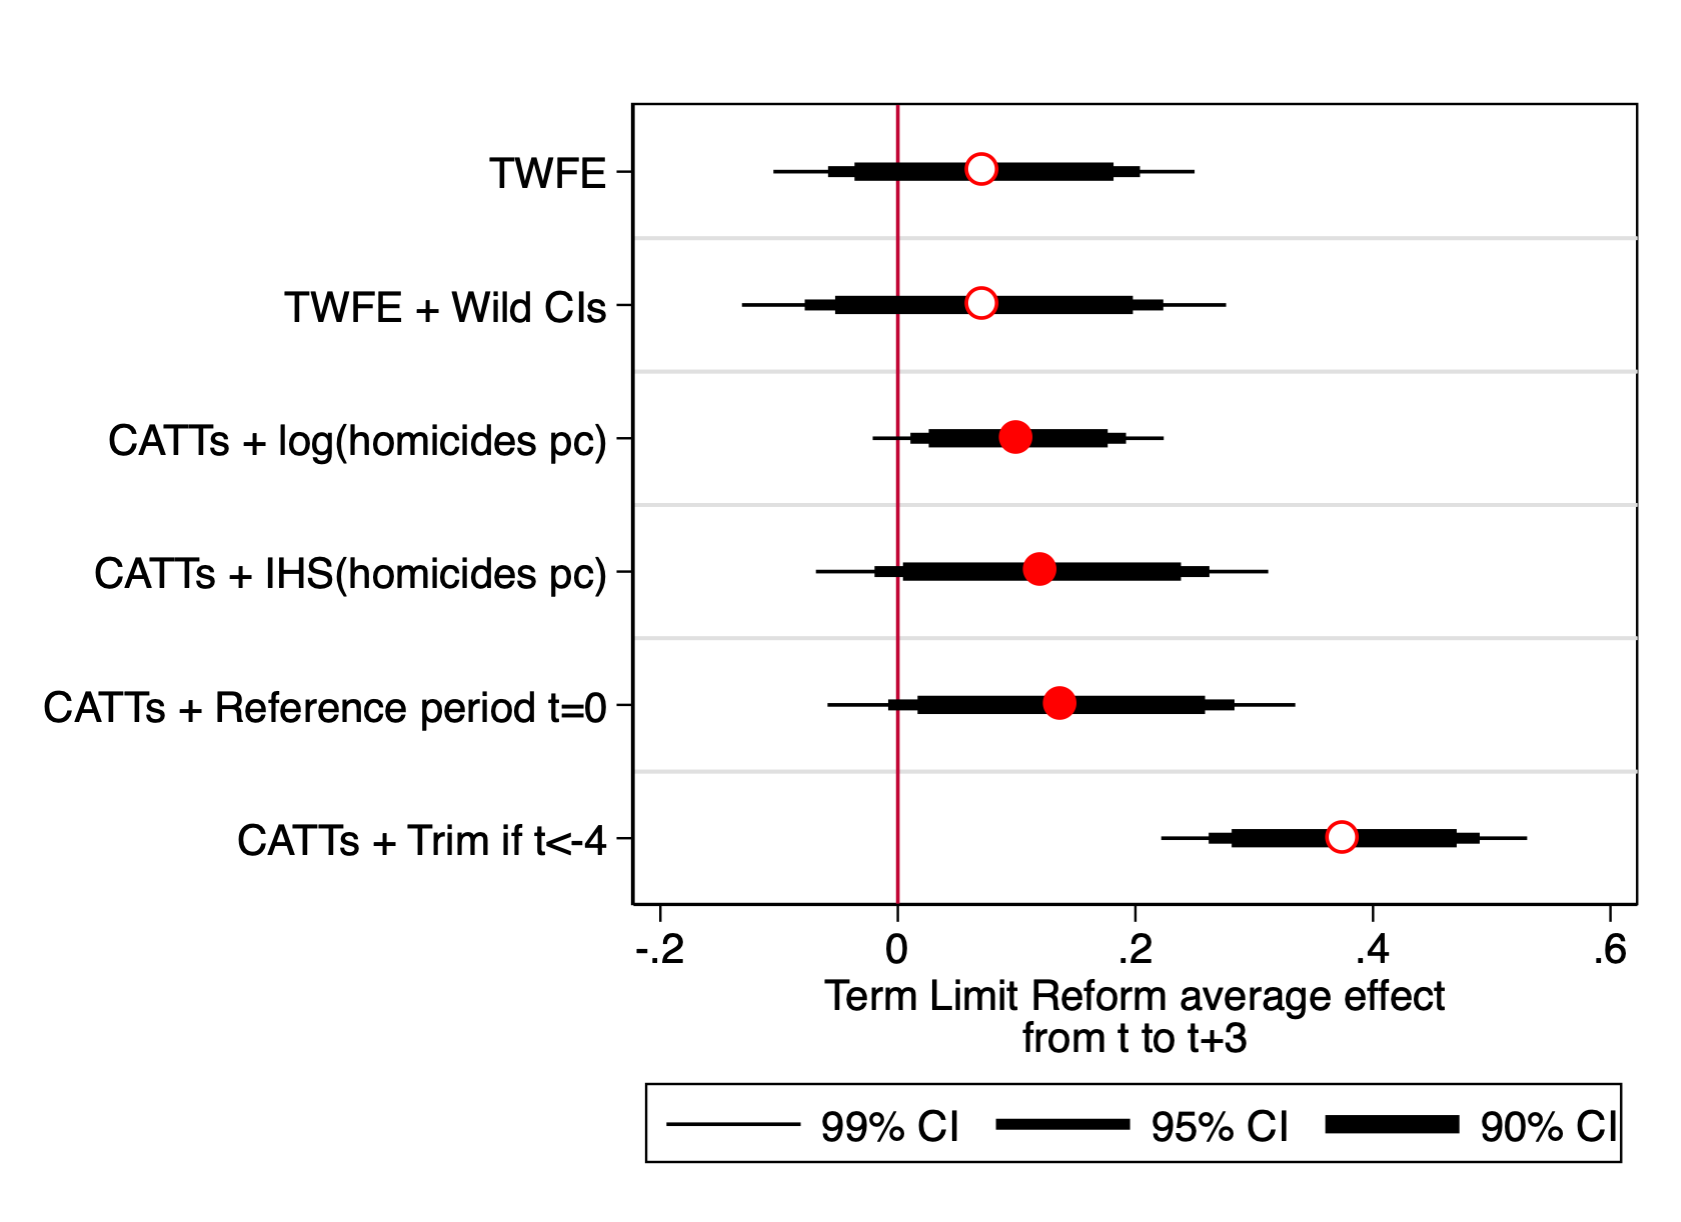
\includegraphics[width=0.7\textwidth]{Chapter1/Figures/average_effects_homicides.png}
       \captionsetup{justification=centering}
       
 \textbf{Note:} Figure \ref{fig:robustness_violence} shows the average treatment effect from t to t+3 across multiple specifications. This average effect was estimated using the IW estimators following \citet{abraham_sun_2020} for each lead and lag relative to the first year a municipality implemented reelection. Red points show that parallel trends hold, while hollow ones imply pretrends. 
\end{figure}      

\begin{figure}[H] 
\centering
 \caption{Effect of Term Limit Reform on Violence, propensity score matching on pretreatment covariates}
 \label{fig:matching_violence}
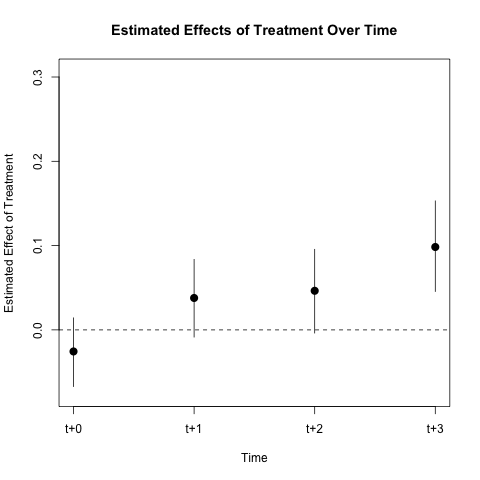
\includegraphics[width=0.75\textwidth]{Chapter1/Figures/panelmatch_logdefuncionespc.png}
       \captionsetup{justification=centering}
    
        
 \textbf{Note:} Figure \ref{fig:matching_violence} produced by propensity score matching that adjust for the treatment and covariate histories during the 5 year periods prior to the treatment. I report 95\% bootstrap confidence intervals clustered at the state level. Covariates include those used to generate Figure \ref{fig:event_study_agreements}. 
 
\end{figure}   
           
    
    
 \clearpage   
 
 %%%% NO ANTICIPATORY ASSUMPTION   
\section{Validating the no-anticipatory assumption \label{appendix:CDLZ}}

%\renewcommand{\thetable}{C-\arabic{table}}
%\setcounter{table}{0}
% \renewcommand{\thefigure}{C-\arabic{figure}}
%\setcounter{figure}{0}
    
         
One way to address the no-anticipatory behavior is to assume that it can only occur in a fixed window prior to the electoral reform, say of one year, especially since the reform was announced in early 2013. However, for states that implemented reelection later this fixed window assumption would not suffice. In other words, only those early adopters of the reform would show unbiased estimates. Late adopters, however, would anticipate the term limit removal an act accordingly biasing the results upwardly.  
 
Another way to assess the no-anticipatory behavior from incumbents in this setting is test whether early vs late adopters differed in their estimated effects. Appendix Figure \ref{fig:CDLZ_agreements} presents \citet{cengiz_etal_2019} ``event-by-event analysis" that estimates treatment effects for each treated Mexican state (28 states) in the sample. States color differs if they are early (2015, red color) or late adopters (2016-2018, blue color). Specifically, I create state-event specific panel datasets and estimate state-specific estimates using separate regressions for each state. Each state dataset contains the treated state and all other states that never received treatment or received treatment after the sample window of $t+1$. For each state I estimate the following DiD regression: 
   
\begin{equation}
y_{mt}=\mu_m	 + \mu_t + \gamma Reform_{mt} + \epsilon_{mt}
\end{equation}

where $Reform_{mt}$ is an indicator variable that takes the value of 1 if the state implemented reelection. If there was evidence of strong incumbent anticipatory behavior, conditional on state covariates such as governor winning margin and alignment with Federal Executive, we would expect strong color clustering across similar estimated effects. In other words, if there is an endogenous response by states to implement the electoral reform, we would see that the positive (or negative) treatment effect would be only by those that implemented reelection earlier or later (events with the same color would be clustered). However, as seen in Appendix Figure \ref{fig:CDLZ_agreements}, this is not the case: there is wide variation in estimated coefficients across early (red) and late (blue) adopters of the reform, conditional and unconditional on state covariates. One would be concerned of the five blue states clustered in the positive end. However, if there was anticipation in these states they would only represent a downward bias of the main results found on the paper.  

\begin{figure}[h]
\centering
\caption{``Event-by-event analysis'' following \citet{cengiz_etal_2019}\\ -95\% confidence intervals-} 
\label{fig:CDLZ_agreements}
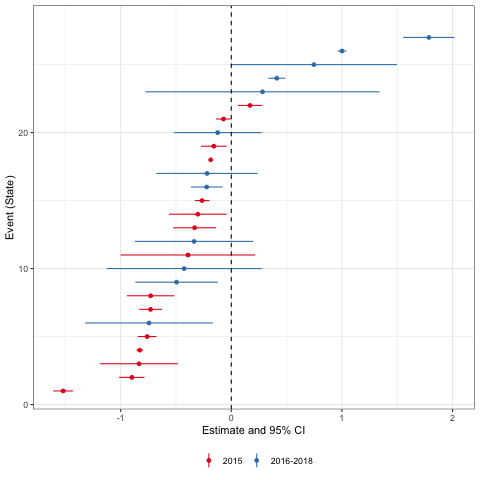
\includegraphics[width=0.5\textwidth]{Chapter1/Figures/CDLZ_cov_acuerdo.png}
       \captionsetup{justification=centering}
       \\
 {\textbf Note:} Estimate separate treatment effects for each event, i.e. each Mexican state in the sample. Each event dataset contains the treated state and all other states that never received treatment or received treatment after the sample window ($t+1$).   
\end{figure}     
   
For robustness, Appendix Figure \ref{fig:stacked_wcontrols_agreements} presents the ``stacked dataset analysis" from \citet{cengiz_etal_2019}. I take each of the ``event-by-event'' datasets from the Appendix Figure \ref{fig:CDLZ_agreements}, stack estimates by cohort and estimate one set of lead and lag variables not using prior treated units as controls. Appendix Figure \ref{fig:stacked_wcontrols_agreements} shows that conditional on state-level covariates, there is strong evidence of parallel trends as well as negative effect of reelection on delegation, but noisy.
       
    
\begin{figure}[H]
\centering
\caption{``Stacked dataset analysis'' following \citet{cengiz_etal_2019}\\ -95\% confidence intervals-} 
\label{fig:stacked_wcontrols_agreements}

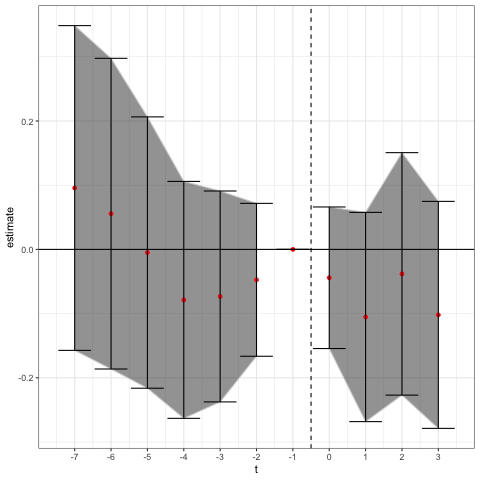
\includegraphics[width=0.5\textwidth]{Chapter1/Figures/stacked_dataset_wcontrols_acuerdo.png}
       \captionsetup{justification=centering}
       \\
 {\textbf Note: Utilize estimated coefficients from Figure \ref{fig:CDLZ_agreements} and stack them in relative time, and estimate lead and lag variables to treatment following the event-by-event analysis setup, i.e. without treatment containment from using prior treated units of controls. Analysis done stacking at the cohort level, and adding municipality and year fixed effects, and clustered standard errors at the state level.}     
\end{figure}   

